% #############################################################################
% This is Chapter 6
% !TEX root = main.tex
% #############################################################################
% Change the Name of the Chapter i the following line
\fancychapter{Personalization \& Customization}
\clearpage
% The following line allows to ref this chapter
\label{chap:chap006}

\section{Introduction}
\label{sec:chap006001}

Artificial Intelligence (AI) systems are showing an increasing promise for numerous healthcare applications.
Recently, the advantages of Deep Learning (DL) are spawning AI systems with human-like performance in several clinical domains~\cite{CALISTO2022102285, Hannun2019, Ruamviboonsuk2019, Stephansen2018}.
However, these applications are not designed to capture the variability of personal or subpopulation level of clinicians ({\it e.g.}, interns, juniors, middles, and seniors)~\cite{Uddin2019}.
In fact, recent works are highlighting how AI and the advancement of technologies together are empowering the aim of personalized and precision medicine~\cite{Subramanian2020, HO2020497, Wetzstein2020}.
Given the need of personalizing and customizing the AI recommendations, an important question in the design of AI systems is how they should communicate (Figure~\ref{fig:fig097}), considering the professional experience of the clinician.

\begin{figure}

\includegraphics[width=\textwidth]{fig097}
\caption[]{A sample of ``Non-Assertive'' ({\it e.g.}, suggesting ``it looks like'') {\it vs.} ``Assertive'' ({\it e.g.}, imposing ``must'') communications.}
\label{fig:fig097}
\end{figure}

As the means to achieve a more persuasive and reliable intelligent agent, we need to analyze and collect data regarding the clinician's behavior~\cite{PELAU2021106855}.
Communication is essential to increase the reliability of an intelligent agent~\cite{10.1145/3311350.3347162} providing a diagnosis to a clinician.
One way to achieve that is by aligning the levels of assertiveness~\cite{pacheco2019alignment} of the agent with the years of experience of the clinician.
Besides that, providing an explanation of `how' and `why' the AI assistant achieved a certain output increases trust on the system, solving a problem known as the ``black-box'' problem~\cite{10.1145/3491102.3502104, CALISTO2021102607}.

In this paper, we present our study for applying {\it BreastScreening-AI} (Section~\ref{sec:app001004}) in two conditions, where clinicians will interact with conventional and assertiveness-based intelligent agents~\cite{pacheco2019alignment, 10.1145/3311350.3347162}.
The assistant will act as a second reader, resulting in improvements in diagnostic performance, by reducing false-positives and false-negatives ({\it i.e.}, Over-Diagnosis {\it vs} Under-Diagnosis), as well as in efficiency and efficacy in the clinical workflow (Section~\ref{sec:app001005}).
While considerable work has focused on improving the accuracy of AI algorithms, comparatively less work focused on improving adoption and usability of interactive assistance techniques.
This paper contributes broadly to the latter by examining what clinicians need when using AI-powered assistance, the practices they adopt while using diagnostic tools, and how these tools affect the end-user attitudes towards the underlying AI algorithms.

Here, we detail a within-subject study with 52 clinicians who interacted with both conventional and assertiveness-based agents, diagnosing a total of 35 patients from a dataset of 289 patients, out of which 34\% have benign abnormalities, 31\% have malignant abnormalities, and the other 35\% are healthy patients (Section~\ref{sec:app001001}).
Two different tones were used to communicate the AI recommendations in our assertiveness-based agent, from a more suggestive to a more imposing tone.
Moreover, the assertiveness-based agent explained `{\it how}' and `{\it why}' the AI algorithms achieved a particular diagnostic by providing human-interpretable clinical arguments for the achieved outputs.

While we used real AI outputs and clinical arguments curated from human clinicians, the AI models were trained for classification and segmentation purposes through different architectures~\cite{HANCER2023321}.
Specifically, through a DenseNet model~\cite{8721151} for a multimodal diagnosis of MammoGraphy (MG) and UltraSound (US) images.
Similarly, a 3D ResNet model~\cite{Aldoj2020} was trained to diagnose the Magnetic Resonance Imaging (MRI) volumes.
Our findings suggest that explaining the AI outputs and clinical arguments by exploring how to adapt the communication through an assertiveness-based agent can benefit AI assistance of medical reasoning.

The novelty of this work is in the application of communication theories through the use of DL systems.
Our goal was to explore and understand how assertiveness-based AI mediation is affecting different expertise levels in a high-stake decision-making domain, such as critical medical decisions dealing with the life of a patient.
For that purpose, we updated the design of the {\it BreastScreening-AI} framework~\cite{CALISTO2022102285} in where we aim to study how does different expertise levels in clinical scenarios are influenced by an assertiveness-based communication.
Not only we are contributing with knowledge of computational interaction approaches in the HCI filed ({\it i.e.}, assertiveness-based AI mediation), but also understanding on how to design interactive systems underpinned by computational principles to the CHI community.

\noindent
In sum, the main contributions of this work are as follows:

\vspace{0.5mm}

\begin{enumerate}
\item We present a novel approach for personalizing and customizing the AI-assisted medical reasoning, providing evidence that assertiveness-based agents can alter clinical workflows by effectively adapting the communication depending on the categories of medical professional experience.
\item We demonstrate that while explaining the AI outputs can contribute to enhancing medical efficiency, its impact heavily depends on the communication tone ({\it i.e.}, more suggestive or imposing the AI recommendations) of the provided clinical arguments.
\item We report our results demonstrating that these assertiveness-based agents can increase the utility of clinical information found and increase user trust in the AI recommendations, without a loss in diagnostic performance.
\item We provide design considerations for adapting the communication in AI-assisted medical reasoning, laying a foundation for future implementations of intelligent agents better capable of personalizing and customizing explanations.
\end{enumerate}

\vspace{0.5mm}

Across the following sections, we outline related works on the issues of guiding the Human-AI Interaction (HAII) topic, assisting clinical decision-making, going through some examples of Clinical Decision Support Systems (CDSS) present in the literature~\cite{NAISEH2023102941, 10.1145/3531146.3533193}, and ending on the effects of AI communication.
We then introduce the design of our {\it Assertiveness-based BreastScreening-AI} assistant, followed by our research questions, hypotheses, and methods.
Last, we report our quantitative and qualitative findings, as well as concluding with a discussion of design considerations.

\section{Related Work}
\label{sec:chap006002}

Medical imaging systems allow the end-user to diagnose several modalities, such as MG, US, or MRI, from a seamless retrieval of medical imaging data~\cite{faraji2019radiologic}.
Bringing those modalities together offers new possibilities for quantitative imaging and diagnoses, but also requires specialized data handling, post-processing, and novel visualization methods~\cite{Igarashi:2016:IVS:2984511.2984537}.
In the clinical domain, medical imaging tools can help experts make better decisions, {\it e.g.}, by identifying cancer prognostics among the available multi-modal data~\cite{IBRAHIM2019438, Tan2023}.
In this document, we focus on understanding different aspects and expectations of a medical imaging CDSS integrated into the radiology workflow.
In particular, our work demonstrates how an assertiveness-based interaction can improve the medical imaging diagnosis.

\subsection{Human-AI Interaction}
\label{sec:chap006002001}

Intelligent agents need to provide users with, not only results, but also accounting for their behaviors during decision-making~\cite{10.1145/3313831.3376807}.
In the field of Human-Computer Interaction (HCI), the topic of eXplainable-AI (XAI) contains subjects that intersect cognitive psychology, learnability, and context awareness~\cite{doi:10.1073/pnas.1618211113, doi:10.1080/07370024.2021.1977128}.
Cognitive psychology is a subject focusing more on explanation theory~\cite{10.1093/mind/fzu023}.
For cognitive psychology, Lombrozo~\cite{LOMBROZO2010303} found that cognitive explanations are strongly connected with causality reasoning.
Learnability is an important part of usability~\cite{10.1145/1753326.1753552}.
Here, Abdul~\cite{10.1145/3173574.3174156} summarized topics of learnibility related for designing a XAI system, such as hints, guidance, and visualizations.

Finally, explainable context awareness is a simplistic representation of the context to inform users what is obtained and which action will be done by the system~\cite{10.1145/3313831.3376545}.
Dey et al.~\cite{10.1145/1518701.1518832} designed a tailored interface, providing visual and textual explanations following several context-aware rules.
However, research in both HCI and AI communities is oftenly disconnected between the two fields~\cite{10.1145/3173574.3174156, 10.1145/3313831.3376807}.
There is a research gap that is not crossing nor combining both fields to the interdisciplinary approach of accounting user's different behaviors during decision-making.

HAII incorporates human feedback in the model training process to create better Machine Learning (ML) models.
In this document, we refer to the topic as HAII, that somehow is addressed by Amershi et al.~\cite{10.1145/3290605.3300233} providing a set of design guidelines~\cite{10.1145/3132272.3134111}.
The work of Kocielnik et al.~\cite{Kocielnik:2019:YAI:3290605.3300641} is also addressing the study on the impact of several methods of expectation setting, and others studied the design for specific HAII scenarios~\cite{aha2017ai}.
While much of the mentioned prior work has employed handcrafted features~\cite{10.1145/3290605.3300233, Kocielnik:2019:YAI:3290605.3300641}, we leverage the rich image data features automatically learned from DL algorithms.

Many researchers have argued that HAII would be improved if the AI systems could {\it explain their reasoning}~\cite{10.1145/3411764.3445717, Rudin2022, Kawamleh2022}.
In medicine, explaining predictions from AI models is particularly salient, where the uncovered patterns of the model can be more important than prediction performance~\cite{Lundberg2020}.
Lundberg et al.~\cite{Lundberg2018} are demonstrating how to retain interpretability by developing a method to provide explanations of model predictions.
Although these works are exploring how clinicians interact with AI recommendations and their perceptions of AI outcomes, they are not taking into account cognitive bias in decision-making.
One of the most notorious cognitive differences is seen between people with different levels of expertise and knowledge~\cite{https://doi.org/10.1111/nuf.12430, Seidel2021}.
It is why we are studying how assertiveness-based agents are designed to adapt their communication tone based on expertise levels to reduce cognitive bias.

\subsection{Assisting Clinical Decision-Making}
\label{sec:chap006002002}

Although the research in interaction with intelligent agents is recent~\cite{burr2018analysis}, still this topic has seen new advances, {\it e.g.}, chat-bots and other agents~\cite{miller2019intrinsically}.
Recent advances in medical technologies that promote the generation of data have continued to drive interaction research in the clinical domain~\cite{azuaje2019artificial, Lopes:2017:UHC:3143820.3144118}.
Moreover, the new interest of the medical community to support AI research projects and the available public {\it datasets}, are encouraging researchers to work in both fields~\cite{lau2018dataset}.
Therefore, we bring together both HCI and AI communities to leverage the high-stakes of clinical decision-making.

The introduction of technology for assisting clinical decision-making is fraught with challenges and unintended consequences, such as critical decisions dealing with patient safety, clinician fatigue, and increased medical errors~\cite{10.1093/jamia/ocab291, 10.1117/12.2613082, doi:10.1148/radiol.212631}.
Moreover, clinicians find AI systems challenging to use because they may have limited technical skills for the adoption of these novel technologies, where these technologies are not customized to behavioral aspects of clinicians~\cite{CALISTO2022102922}.
In fact, the AI outcomes are challenging to understand and communicate to clinicians, as these systems often have poorly designed interfaces~\cite{10.1145/3555157}, without taking into account differences of clinician's characteristics during decision-making.
For instance, the reasoning of a novice clinician vary from an expert~\cite{Edgar2022}.

There is a lack of large-scale deployment of these systems in healthcare~\cite{10.1145/3411764.3445432, SU202328, ZAPPATORE20231}, making it difficult to understand how these systems are perceived and used by their intended users in real-world settings.
HCI has proposed and conceptualized several approaches of human-AI relationships, such as interactive Machine Learning (iML)~\cite{10.1145/604045.604056}, Human-In-The-Loop (HITL)~\cite{holzinger2016interactive, 10.1145/3397481.3450668}, human-AI symbiosis~\cite{JARRAHI2018577}, and human-AI collaboration~\cite{10.1145/3411764.3445432}.
However, these approaches mainly use human input to improve the prediction accuracy, model efficiency, and interpretability of AI to the unwanted added burdens on healthcare professionals~\cite{10.1145/3555157, 10.1145/3209889.3209897}.
Wang et al.~\cite{10.1145/3411764.3445432} studied the perception and usage of AI systems for assisting clinical decision-making, but the work is not accounting the potential differences between behavioral reasoning.
Similarly, the work of Panigutti et al.~\cite{10.1145/3491102.3502104} is only considering accurate algorithmic suggestions without considering the clinician's professional medical experience.
In our work, we are covering this literature gap by studying how to personalize and customize algorithmic suggestions to different levels of professional medical experience.

\subsection{Clinical Decision Support Systems}
\label{sec:chap006002003}

In medical applications, DL systems have also been the major contributor to the success of several CDSS applications~\cite{esteva2019guide}.
Such CDSS applications can detect and learn patterns or make predictions to assist clinicians, such as pathologists, or radiologists, among others, in high-stakes clinical decision-making~\cite{10.1145/3555157}.
For instance, on the diagnosis of skin cancer \cite{esteva2017dermatologist}, the segmentation of cardiac MRI \cite{8759179}, or breast cancer detection \cite{MAICAS2019101562}, there are a variety of works where DL systems were introduced for clinical purposes.
Their outstanding performance in identifying meaningful patterns within the available data, recently used to help humans learn new biomarkers of specific diseases \cite{wang2019deep}.
Because of that, several works are arguing that these models can see beyond what a trained radiologist sees in medical images~\cite{mckinney2020international, Rajpurkar2022, MAIERHEIN2022102306}.
Although some works are already contemplating the idea of a CDSS that predicts and explains some AI outcomes~\cite{MAICAS2019101562, CALISTO2022102285}, they ignore the need of adapting the communication tone for a personalized and customized medicine.

Most of the best performing CDSS rely on ML algorithms that learn specific tasks from training data~\cite{10.1001/jama.2018.17163, Zaman49, 10.1145/3399715.3399744}.
The field recently gained enormous interest, primarily due to the practical successes of DL~\cite{10.1007/978-3-030-22871-2_67}.
The rapid and widespread development of DL methods supports a wide range of image analysis tasks in breast cancer diagnosis, including classification, detection, and segmentation \cite{lecun2015deep, DIN2022106073}.
These methods rely on large annotated datasets to learn essential and discriminative image features for each specific task, with performances matching and even surpassing humans \cite{esteva2017dermatologist}.
However, past works are highlighting several obstacles in going from research and development environments to hospital or real clinical settings for these set of applications~\cite{https://doi.org/10.3322/caac.21552, 10.1145/3313831.3376718}.

The lack of utility to clinicians and logistical hurdles that slow or block deployment are frequent obstacles in real clinical settings~\cite{Elwyn2013, Musen2021}.
Even systems with widespread adoption, such as systems to aid radiologists during breast cancer diagnosis, are requiring them to do more work~\cite{KOHLI2018535}.
Instead of reducing the radiologist workload or ease the clinical workflow, these systems are generally not improving the radiologist's diagnostic accuracy~\cite{Cole2014fi, KOHLI2018535}.

%%%%%%%%%%%%%%%%%%%%%%%%%%%%%%%%%%%%%%%%%%%%%%%%%%%
\begin{figure*}[htpb]
\centering
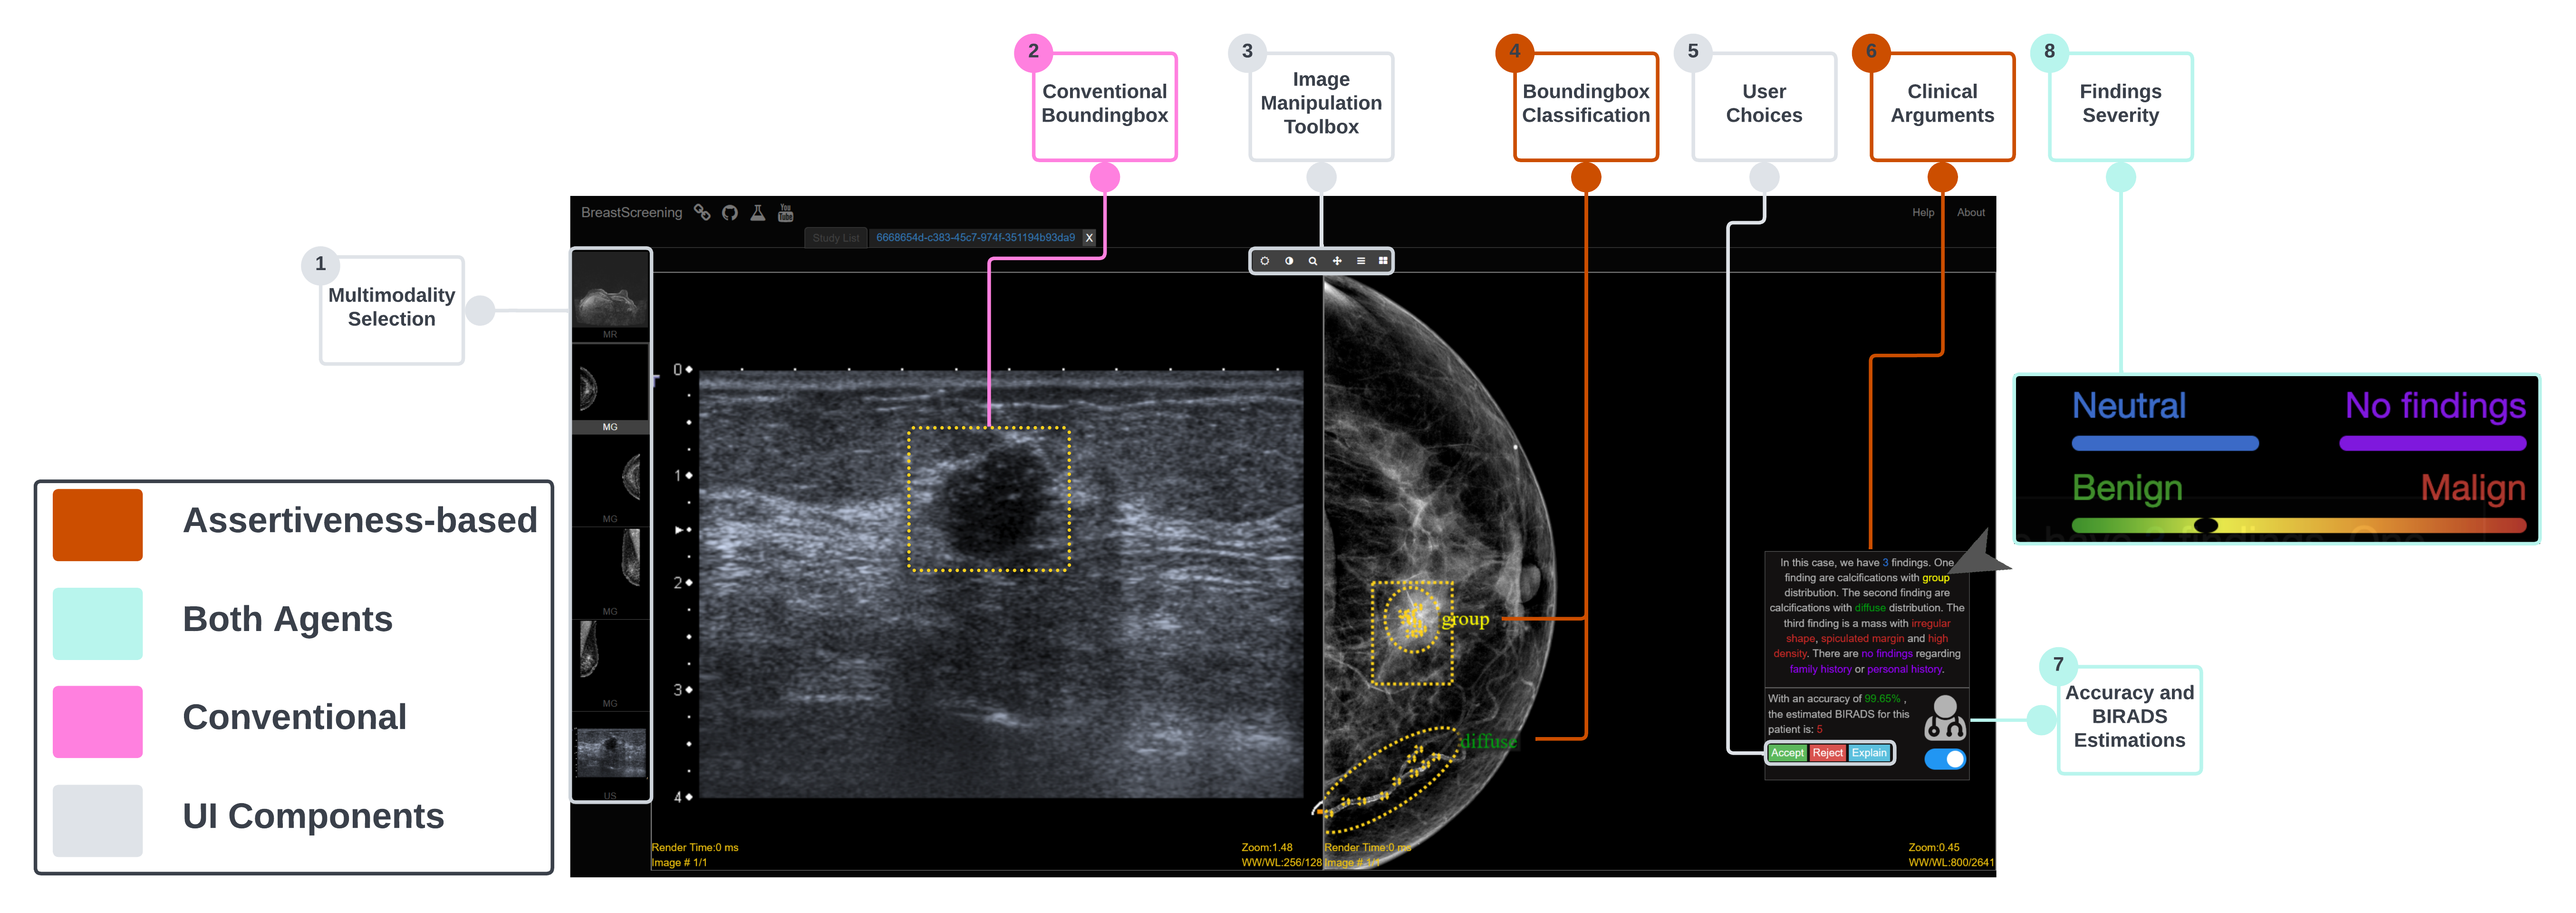
\includegraphics[width=0.935\textwidth]{fig096}
\caption[]{Interface for conventional and assertiveness-based AI agents for medical imaging analysis. Attributes are associated with numbers in each testing condition. When a clinician hovers the mouse over each variable ({\it e.g.}, accuracy, BIRADS, or any other clinical argument of attribute 6), the AI agent will pop up a window to inform the severity of each finding. The colors are ranging from benign (green) to malign (red). The number of findings is a (blue) neutral color, conclusions taken from the interviews, as one highly severe finding can be more critical than having several findings. During the interviews, clinicians choose the purple color for the family and personal history variables of the patient.}
\label{fig:fig096}
\end{figure*}
%%%%%%%%%%%%%%%%%%%%%%%%%%%%%%%%%%%%%%%%%%%%%%%%%%%

The work of Beede et al.~\cite{10.1145/3313831.3376718} studies the introduction of CDSS set of tools, with the primary focus on AI systems that use clinical data.
However, they are not examining the use of real patient AI predictions.
Our work covers this gap by, not only incorporating real granular patient information from the AI outputs, but also studying how to personalize and customize a CDSS for the clinical setting.

Across the HCI literature~\cite{10.1145/3311957.3359433, 10.1145/3359206, Fitzpatrick2013, 10.1145/3538882.3542790}, or more precisely, from the CHI community~\cite{10.1145/3313831.3376718, 10.1145/3290605.3300234}, human-centered evaluation of interactive, DL systems, is an open area of research within clinical environments.
Cai et al.~\cite{10.1145/3290605.3300234} created interactive techniques, leading to an increased diagnostic utility and user trust in the predictions from a DL system, used by clinicians in a lab setting.
Correspondingly, Cai et al.~\cite{10.1145/3359206} examined in the lab setting what information clinicians found to be important when being introduced to AI assistants, before integrating these assistants into routine prostate cancer screening practice.
While these works bring us closer to understand the clinician's needs as they interact with DL-based systems, they do not account for the heterogeneous behavioral nature of decision-making.

\subsection{Effects of AI Communication}
\label{sec:chap006002004}

Trust is critical in communication, especially, in clinical environments, where clinicians are exposed to critical scenarios that affect life decisions~\cite{Amann2020}.
From the HCI literature~\cite{10.1145/3479587, 10.1145/3334480.3375147, 10.1145/3334480.3382842}, we know that the development of trust is influenced by the positive motivational attribution between the communication entity and the user.
The work of Hohenstein et al.~\cite{HOHENSTEIN2020106190} is showing that a successful collaboration between human and AI occurs when ambiguity and uncertainty in terms of perceptions are reduced through trust~\cite{HOHENSTEIN2020106190}.
While communicating AI predictions and explanations is shaping the design of recent works~\cite{Lundberg2020, 10.1145/1518701.1518832}, we do not know how assertiveness-based AI mediation is affecting novice or expert clinicians.

To avoid unexpected clinical consequences, we need to understand the effects of AI communication on human interactions.
In fact, the direct effects of communication are suggesting that clinicians' level of trust in an AI system directly affects their perception of the outcomes~\cite{HOHENSTEIN2020106190}.
Panigutti et al.~\cite{10.1145/3491102.3502104} are arguing that higher levels of trust will cause the clinician to have a positive attitude, resulting in high satisfaction and positive perceptions of performance with respect to the interaction outcome.
Moderation via adapting the communication suggests that trust will influence how a clinician interprets and evaluates information relevant to attitude and behavior.
Attribution theory tell us that when behavior is consistent with explanations, humans will attribute causality to self characteristics and needs~\cite{LOMBROZO2010303}.
On the other hand, when behavior is inconsistent with prior expectations, where there is missing information or ambiguity, external cues will determine behavior~\cite{HOHENSTEIN2020106190}.
As an example, a novice clinician asking for help and receiving a suggestive, {\it i.e.}, non-assertive communication.
When in a real human-human interaction, would receive an assertive recommendation from an expert advisor.
The novelty of our work is in the application of assertive communication theories in a deep learning system and clinical scenario that considers its use.

\section{Assertiveness-based System}
\label{sec:chap006003}

In this study, we explore how human-AI interactions are affected by the ability of an AI agent to not only incorporate granular patient information from the AI outputs but also exploring how to adapt the communication tone ({\it i.e.}, more assertive or suggestive) depending on the medical experience ({\it i.e.}, novice or expert) of the clinician.
Specifically, we compare the AI outputs (Figure~\ref{fig:fig096}) that explain to clinicians some clinical arguments with more granular information about the patient regarding the lesion details, to a conventional agent that only provides numeric estimates ({\it e.g.}, BIRADS and accuracy) of the classification.

Our assertiveness-based agent uses recommendations for classifying and segmenting:
(1) the number of detected findings;
(2) the patient severity of each breast and per medical imaging modality;
(3) a visual scale representing the benign or malign estimates;
(4) providing visualization of the sensitivity and specificity outcomes of the models; and
(5) with clinical arguments of the patient, such as pathological co-variables.
To compare the assertiveness-based agent to the conventional agent, we inform participants that the recommendations are generated by our AI models, so that they can also provide some feedback concerning the model performance.

Figure~\ref{fig:fig096} illustrates how the two AI agents were integrated into an existing medical workflow for the classification of medical imaging data on the support of breast cancer diagnosis.
Both agents are recommending classification and segmentation based on the DenseNet model~\cite{8721151} for MG and US, as well as based on the ResNet model~\cite{TALO2019101673} for MRI.
The two AI agents provided the severity classification of the patient via BIRADS~\cite{SPAK2017179}, the accuracy of the model for that classification, and the segmentation of the lesion to explain the regions that derived from that classification.

Clinicians can open the patient by selecting the ID in a list of patients.
When the patient is open (attribute 1 of Figure~\ref{fig:fig096}), clinicians can select each respective image of the breast, by dragging-drop each image to the view-ports.
From here, clinicians can manipulate the image through the toolbox (attribute 3 of Figure~\ref{fig:fig096}).
In the end, the idea is to {\it accept} or {\it reject} the final recommendation of the AI agent (attribute 5 of Figure~\ref{fig:fig096}), while clinicians can also ask for an {\it explanation} to support their final decision-making.
The key difference between the two AI agents was in how they show communication with clinicians.
A typical output from an AI model includes not only the predicted classification of the BIRADS, but also a likelihood distribution over all possible classification choices.

In our study, both AI agents were designed to communicate this type of {\it quantitative} confidence in two ways (Figure~\ref{fig:fig098}):
(1) for the conventional condition, clinicians could simply see the suggested numeric representation of the BIRADS and the respective accuracy of the model;
(2) for the assertiveness-based condition, the agent was communicating the clinical arguments along with the communication of the BIRADS and accuracy, but this time by descriptive information.
While our conventional agent employed this baseline numeric representation of confidence, our assertiveness-based agent is communicating the {\it quantitative} confidence based on a descriptive sentence of the clinical arguments.
Specifically, the image view-port was augmented with an additional bounding box or circle ellipse {\bf highlighting the lesion characteristics} that were likely to explain the final BIRADS classification.
Note that these suggestions did not dictate the order in which imaging modalities are presented to clinicians.
Indeed, clinicians can remain to decide freely what modalities and clinical arguments are reviewed first.

%%%%%%%%%%%%%%%%%%%%%%%%%%%%%%%%%%%%%%%%%%%%%%%%%%%
\begin{figure}[htpb]
\begin{center}
\centering
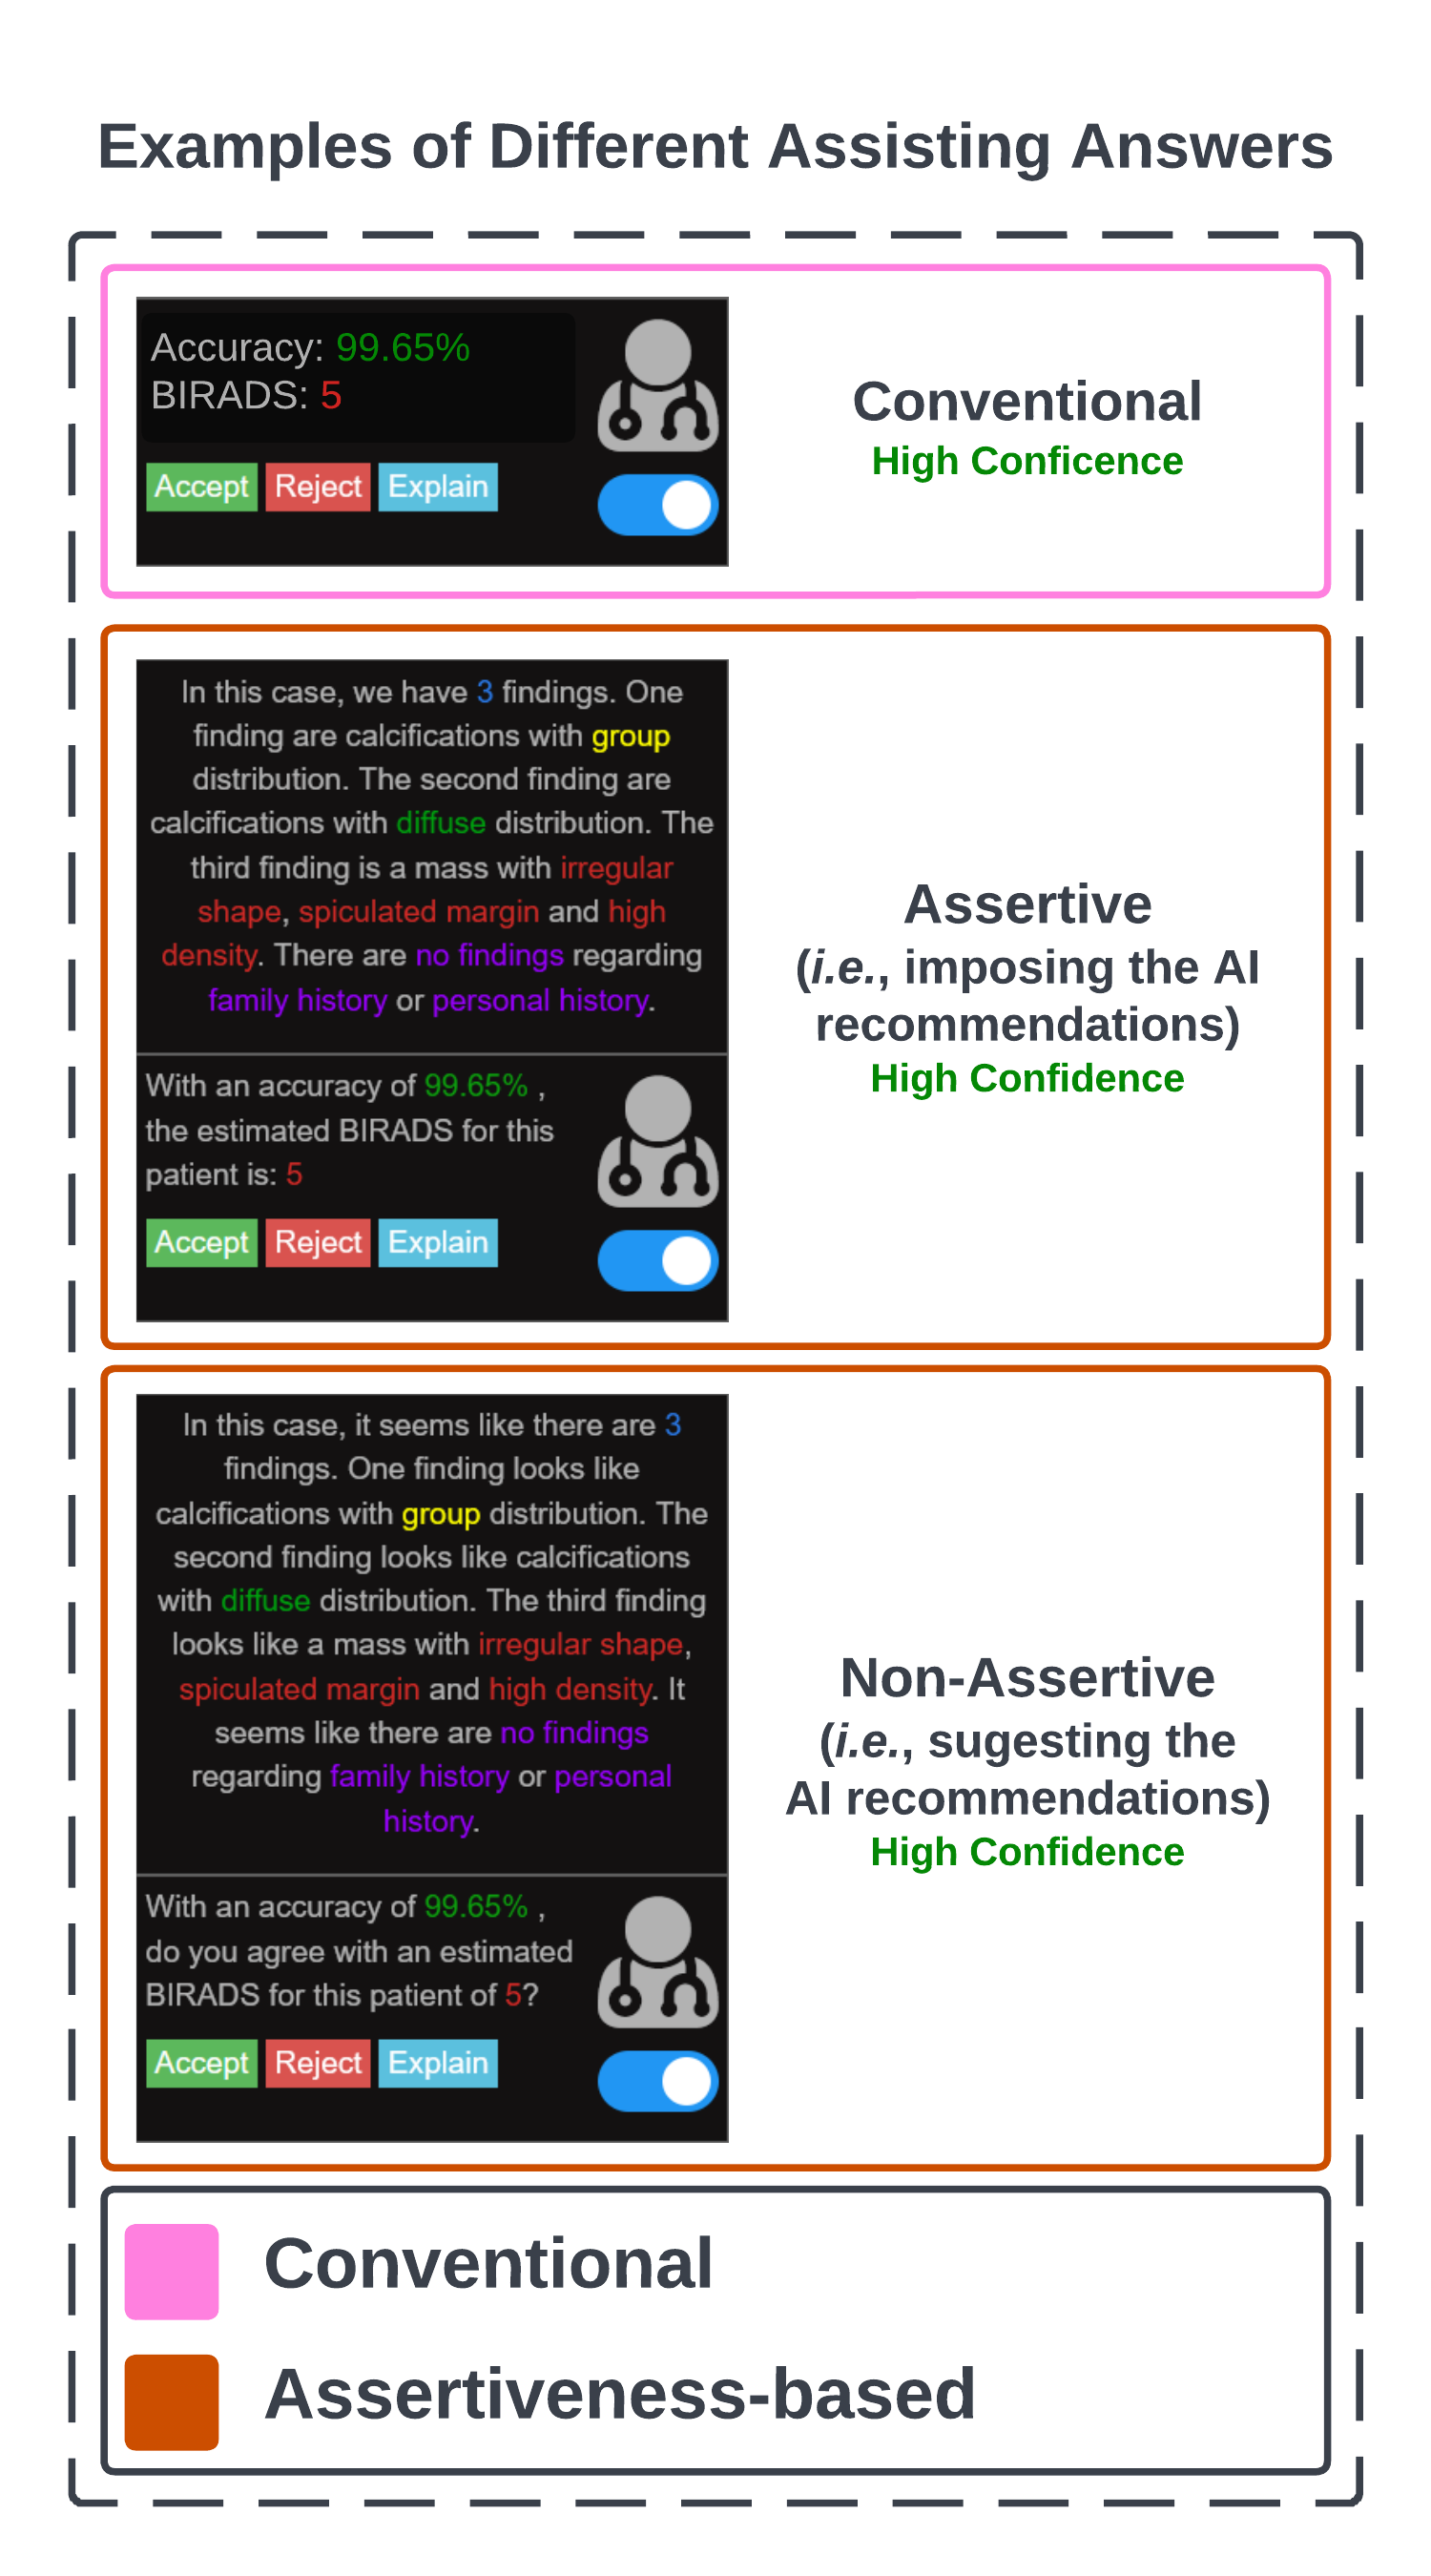
\includegraphics[width=0.625\textwidth]{fig098}
\end{center}
\caption[]{Example of representative use cases for the different testing trials. From top to the bottom, the first agent is representing a conventional example (pink), while the other two are representing assertiveness-based examples (brown), from assertive to non-assertive communication.}
\label{fig:fig098}
\end{figure}
%%%%%%%%%%%%%%%%%%%%%%%%%%%%%%%%%%%%%%%%%%%%%%%%%%%

The patient's detailed augmentation for medical imaging on breast cancer diagnosis was extended with an {\bf assertiveness-based explanation}.
With our system, we are listing human-interpretable clinical arguments for classification and segmentation recommendations that would adapt their communication depending on the personalized and customized demographic characteristics of the clinician.
These clinical arguments correspond to the classification outputs of an AI model and were trained on data (Section~\ref{sec:chap006005002}) from real-world clinical cases, as described next.

\section{Research Questions \& Hypotheses}
\label{sec:chap006004}

The final purpose of our research is twofold.
Through assertiveness-based agents, we first aim to understand how personalized and customized communication could affect medical assessments in terms of the efficiency and efficacy of the clinical workflow.
Secondly, we aim to understand how clinicians perceive assertiveness-based agents differently.
Thus, our work addresses two primary research questions concerning the impact of assertiveness-based agents on efficiency and efficacy (RQ1), as well as the perception (RQ2) of clinicians.

\vspace{2.5mm}

\noindent
Specifically, we consider the following research questions and related hypotheses:

\vspace{0.5mm}

% New RQs
%%%%%%%%%%%%%%%%%%%%%%%%%%%%%%%%%%%%%%%%%%%%%%%%%%%
\begin{itemize}
\item {\bf RQ1.} How does an assertiveness-based agent affect medical assessments?
\begin{itemize}
\item {\bf H1.1.} Efficiency of clinicians in terms of time performance per each diagnosed patient will be higher with an assertiveness-based agent.
\item {\bf H1.2.} Classification accuracy of clinicians will not suffer with an assertiveness-based agent.
% For the H1.3., we have two options:
% In the following H1.3., we will need to say earlier that the personalized explanations are the levels ({\it i.e.}, more or less assertive) of the assertiveness-based communication. So that we can stay aligned with the paper (https://doi.org/10.1145/3313831.3376506) that motivated this work.
\item {\bf H1.3.} Through assertiveness-based communication, accuracy differences between novice and expert clinicians will depend on the tone of the personalized explanations.
% Here, we will be direct to the point. However, we will not be inline of the inspired literature (https://doi.org/10.1145/3313831.3376506) which is motivating this work.
% \item {\bf H1.3.} Differences in accuracy between novice or expert clinicians will depend on the levels ({\it i.e.}, more or less assertive communication) of the assertiveness-based agent.
\end{itemize}
\item {\bf RQ2.} How is an assertiveness-based agent perceived by clinicians?
\begin{itemize}
\item {\bf H2.1.} Clinicians will have a preference for an assertiveness-based agent.
\item {\bf H2.2.} Clinicians will consider an assertiveness-based agent more trustworthy.
\item {\bf H2.3.} Personalized highlights and explanations will not increase clinicians' workload nor decrease usability.
\item {\bf H2.4.} Novice and expert clinicians will perceive reliability and capability differently, depending on the levels of assertiveness.
\end{itemize}
\end{itemize}
%%%%%%%%%%%%%%%%%%%%%%%%%%%%%%%%%%%%%%%%%%%%%%%%%%%

In real-world clinical settings, time of clinicians is a limited and expensive resource that should be reallocated efficiently.
We take the position that while clinicians should make their clinical assessments with care, AI agents can help on the diagnosis efficiency.
Our assertiveness-based agent is designed to summarize the recommendations, and to provide clinical arguments explaining the underlying classification and segmentation of the AI models.

For RQ1, our protection is that personalized and customized explanations can inform clinical decision-making.
Therefore, it will increase clinicians' classification accuracy without reducing their time performance over diagnosis.
Especially, we envision that adapting the communication of the personalized explanations is crucial for successfully informing decision-making of clinicians.

The HCI research community has settled that poor user perception can be a barrier to adoption of technology regardless of performance~\cite{10.1145/3313831.3376506, 10.1145/3479549, 10.1145/3434073.3444649}.
In fact, the user perceptions of preference and trust are essential in predicting technology adoption~\cite{10.1145/3434073.3444649}.
Hence, it is important to investigate clinicians' perception, as we do in RQ2.
Beyond the primary outcome in terms of reliability in AI-assisted clinical assessments, our goal is also to understand how assertiveness-based agents are perceived by clinicians.

\section{Methods}
\label{sec:chap006005}

As a way to improve clinical decision-making, the goal of our study is to attain a deeper understanding of personalized and customized mechanisms, exploring how to adapt the communication of agents depending on the medical experience of clinicians.
Our study draws from 52 semi-structured interviews and user testing with clinicians for breast cancer detection via medical imaging diagnosis.
To accomplish this goal, we conducted a two-condition study, within-subjects, counterbalanced experiment, in which each subject participated in three trials, providing us with rich information to analyze.

Interviews were conducted from March 2022 to June 2022.
Research questions were fused from these interviews and observations, thanks to the support of user-centered activities, such as workshops, focus groups, affinity diagramming, data clustering, and prototype co-design, leading us to reported problems.
Participants in these sessions include clinicians from different healthcare institutions, researchers from the ML field, and HCI researchers.
Before the work commenced, the study was approved by the ethics committee of each clinical institution.
Next, we describe the details of our controlled experiment including the task, dataset, information of participants, study procedures, and statistical analysis.

\subsection{Task}
\label{sec:chap006005001}

We conducted our study in the field of imaging classification on breast cancer, a clinical domain with typically high False-Positive rates to over-diagnose a patient~\cite{KIM2020e138, doi:10.1377/hlthaff.2014.1087}.
In particular, we compared our conventional and assertiveness-based agents in the context of assisting trained medical personnel in the task of a breast cancer diagnosis.
For the conventional condition, we used the {\it BreastScreening-AI} framework~\cite{CALISTO2022102285} publicly available (\href{https://mida-project.github.io/prototype-multi-modality-assistant/}{git.io/JMjDi}) and built for the development of medical assistants.
Aside from the already available functionalities of this framework, we developed two conditions for testing our hypothesis from a post-hoc analyses concerning how to personalize and customize the AI outcomes to clinicians.
We raised several trials, from a more suggestive (non-assertive) to a more assertive tone of the AI recommendations, where clinicians with different levels of expertise are interacting with both trials and the conventional.
In the end, all clinicians interacted with one conventional, one non-assertive, and one assertive agent.
Each clinician diagnosed three patients with different severities, where the task was to {\it accept} or {\it reject} the AI recommendations.

There are two groups of clinicians with different medical professional experiences:
(a) novice; and
(b) expert.
Patients are divided into three groups of breast severities:
(i) low severity, representing the BIRADS of 1, meaning there are no findings for that patient and both breasts are healthy;
(ii) medium severity, representing the BIRADS of 2 and 3, meaning there are some findings with higher probability of benign suspicious; and
(iii) high severity, representing the BIRADS of 4 and 5, meaning there are findings with higher probability of malign suspicious.
Usually, each patient has available three types of modalities ({\it i.e.}, MG, US, and MRI).
For this task, clinicians need to read six imaging views approximately per each patient:
(1) one CC-L;
(2) one CC-R;
(3) one MLO-L;
(4) one MLO-R;
(5) one US; and
(6) one DCE-MRI volume with between 100 and 200 frames.
Shortly, clinicians participated as readers while assessing each patient in terms of the likelihood and location of the malignancy.

During the task of responding to the lesion localization, the reader clinician provides the severity classification of the clinical argument for that suspicious attribute on the image.
For each image, the clinician classifies the patient final severity assessment via BIRADS classification by default.
Meaning that, although the patient has some clinical arguments ({\it e.g.}, group microcalcifications with diffuse distribution in Figure~\ref{fig:fig098}) pointing to a BIRADS of 2, if there is a suspicious irregular shape mass with spiculated margin, by default the clinician will consider the final BIRADS as a 5.

The task of diagnosing breast cancer involves reading heterogeneous appearances, ranging from obvious masses with spiculated margins to subtle asymmetric or faint microcalcifications~\cite{Sturesdotter2020}.
This leads to difficulties for clinicians in achieving an accurate diagnosis and consistent interpretation of the patient.
Because of that, clinicians apply rules from radiological guidelines to classify breast images based on visually inspecting the patterns on the image~\cite{doi:10.1148/radiol.2020192534}.

The classification of breast cancer via the BIRADS scale lends itself to a task for our study on AI agents in medical imaging assessments.
Not only the task is a time-consuming and tedious procedure for clinicians, but also relies on non-trivial classification tasks.
Indeed, the prior medical literature has established that the medical error of clinicians has between 50\% and 30\% chance of being a false-positive and about 10\% chance of being a false-negative~\cite{10.1093/jbi/wbaa118}.

\subsection{Dataset}
\label{sec:chap006005002}

In this paper, we used a total of 338 cases acquired in the first hospital (Section~\ref{sec:chap006005003}).
From this set of cases (Section~\ref{sec:app001002}), 289 were classified by the head of radiology.
Each patient has several images concerning four X-ray mammography (two in CC and two MLO views), one ultrasound image to train the DenseNet model, and roughly DCE-MRI images in MRI to train the ResNet model.
In the MRI volumes, we take several image slices per patient, where the lesion is present.
This provides us roughly 2890 images ({\it i.e.}, 289~\texttimes~(4 + 1 + 5)), that are used to train/test the AI models.

Traditional image processing and deep learning techniques require extensive pre-processing~\cite{Zhong_2020}.
As a matter of fact, it is known that a cleaning dataset is welcome when training a deep neural network~\cite{RIASATIAN2021102032}.
In our study, this stage is of the utmost importance, since the MG, US, and MR images contain quite different intensities and the images are of different sizes.
Thus, before introducing the images to the DenseNet and ResNet models, we pre-process the data (Section~\ref{sec:app001006}).
Specifically, we perform data normalization, so that the images have the same intensity, regardless of the modality.

All the images are resized to 224x224 pixels.
The images are normalized by subtracting their mean and dividing by their standard deviation.
The above size is used since the DenseNet model is prepared to receive the input with this format.

\subsection{Participants}
\label{sec:chap006005003}

We recruited 52 clinicians as participants for our study on a volunteer basis from a broad range of clinical environments, including different health institutions (public hospitals, cancer institutes, and private clinics).
Our clinicians were recruited through the already established protocols under this study from 11 different clinical institutions: (1) \href{https://hff.min-saude.pt}{Hospital Prof. Dr. Fernando Fonseca (HFF)}; (2) \href{https://www.ipolisboa.min-saude.pt}{Instituto Portugu\^{e}s de Oncologia (IPO) de Lisboa (IPO-Lisboa)}; (3) \href{https://www.chln.min-saude.pt}{Hospital de Santa Maria (HSM)}; (4) \href{http://www.ipocoimbra.min-saude.pt}{IPO de Coimbra (IPO-Coimbra)}; (5) \href{http://www.madeiramedicalcenter.pt}{Madeira Medical Center (MMC)}; (6) \href{https://www.sams.pt}{Serviços de Assist\^{e}ncia M\'{e}dico-Social do Sindicato dos Banc\'{a}rios do Sul e Ilhas (SAMS)}; (7) \href{http://www.chbm.min-saude.pt}{Hospital do Barreiro (HB)}; (8) \href{https://www.chporto.pt}{Hospital de Santo Ant\'{o}nio (HSA)}; (9) \href{https://www.fchampalimaud.org/}{Champalimaud Foundation (CF)}; (10) \href{https://www.chtmad.min-saude.pt/}{Centro Hospitalar De Tr\'{a}s-Os-Montes E Alto Douro, E.P.E. (CHTMAD)}; and (11) \href{https://www.chlo.min-saude.pt/}{Centro Hospitalar de Lisboa Ocidental. EPE (CHLO)}.
All clinicians and clinical institutions gave prior permission to use their data for research purposes under this study.

From the demographic questionnaires (Section~\ref{sec:app001003}), 55.77\% of participants are expert clinicians, whereas 34.62\% are seniors having more than 10 years of practical experience, and 21.15\% are middle clinicians having more than 5 years but less than 10 years.
Similarly, 44.23\% of participants are novice clinicians, whereas 32.69\% are juniors after taking the exam, having up to 5 years of clinical experience, and 11.54\% are interns before the medical specialty exam.
Each clinician was exposed to the three trials ({\it i.e.}, conventional, assertive, and non-assertive) in a counter-balanced manner.

\subsection{Procedure}
\label{sec:chap006005004}

After providing an informed consent form for participation in the study, each clinician reported information concerning several self-characteristics.
First, they reported their demographic characteristics (Section~\ref{sec:app001003}).
Second, they reported their professional backgrounds, such as clinical education ({\it i.e.}, radiology, surgery, nurse, technician, etc), areas of expertise, work sector, and medical experience.
Finally, information about their experience while reading medical imaging data.
Next, clinicians familiarized themselves for about 3 minutes with our user interface and with the basic functionalities common to both AI agents.

At this stage, each participant interacted with the assistant, {\it accepting} or {\it rejecting} the system suggestion in the two different conditions: (a) conventional; and (b) assertiveness-based.
The set of patients was providing participants 289 patients, while all patients must have at least one of the three available modalities.
Each participant open the set of three patients ({\it e.g.}, {\bf P1}, {\bf P2} or {\bf P3}), chosen randomly, and examined it.
During the examination, the participant interacts with the available functionalities of the system.

Clinicians performed the same task of diagnosing three patients twice, once with the conventional agent and another time with the assertiveness-based agent.
For each task, clinicians were asked to read the suggested AI recommendations, where the task ends when clinicians {\it accept} or {\it reject} the proposed BIRADS.
Additionally, clinicians could ask for a visual {\it explanation} inside the image during the task.
The list of patients was fully classified by the AI models, and clinicians could revise the explanations (bounding boxes 2 and 4 of Figure~\ref{fig:fig096}) for the important regions to consider.

After each task, clinicians filled out a brief feedback questionnaire exploring their perception of each AI agent.
The questionnaire included scales to measure three dimensions of trust~\cite{Loper2020} represented by perceived understanding, competence, and thoughtfulness, as well as cognitive workload by using NASA-TLX~\cite{info:doi/10.2196/19472}, and usability by using SUS~\cite{doi:10.1080/10447318.2018.1455307}.
With these measures, our purpose was to understand perceived diagnostic utility and decision-making support provided by the AI agents, and whether clinicians thought they would use the agents in practice.
Upon completing all the tasks, we measure the preferences while using both conventional or assertiveness-based agents, and the different levels of assertiveness.

Clinicians compared both AI agents with respect to reliability, capability, and overall preference.
To measure the levels of assertiveness rated between novice and expert clinicians, we measured the reliability and capability of the different ({\it i.e.}, from more suggestive to more imposing AI recommendations) communication tones of the assertiveness-based agent.
Clinicians rated these items on a 7-point Likert scale.

%%%%%%%%%%%%%%%%%%%%%%%%%%%%%%%%%%%%%%%%%%%%%%%%%%%
\begin{figure*}[htpb]
\centering
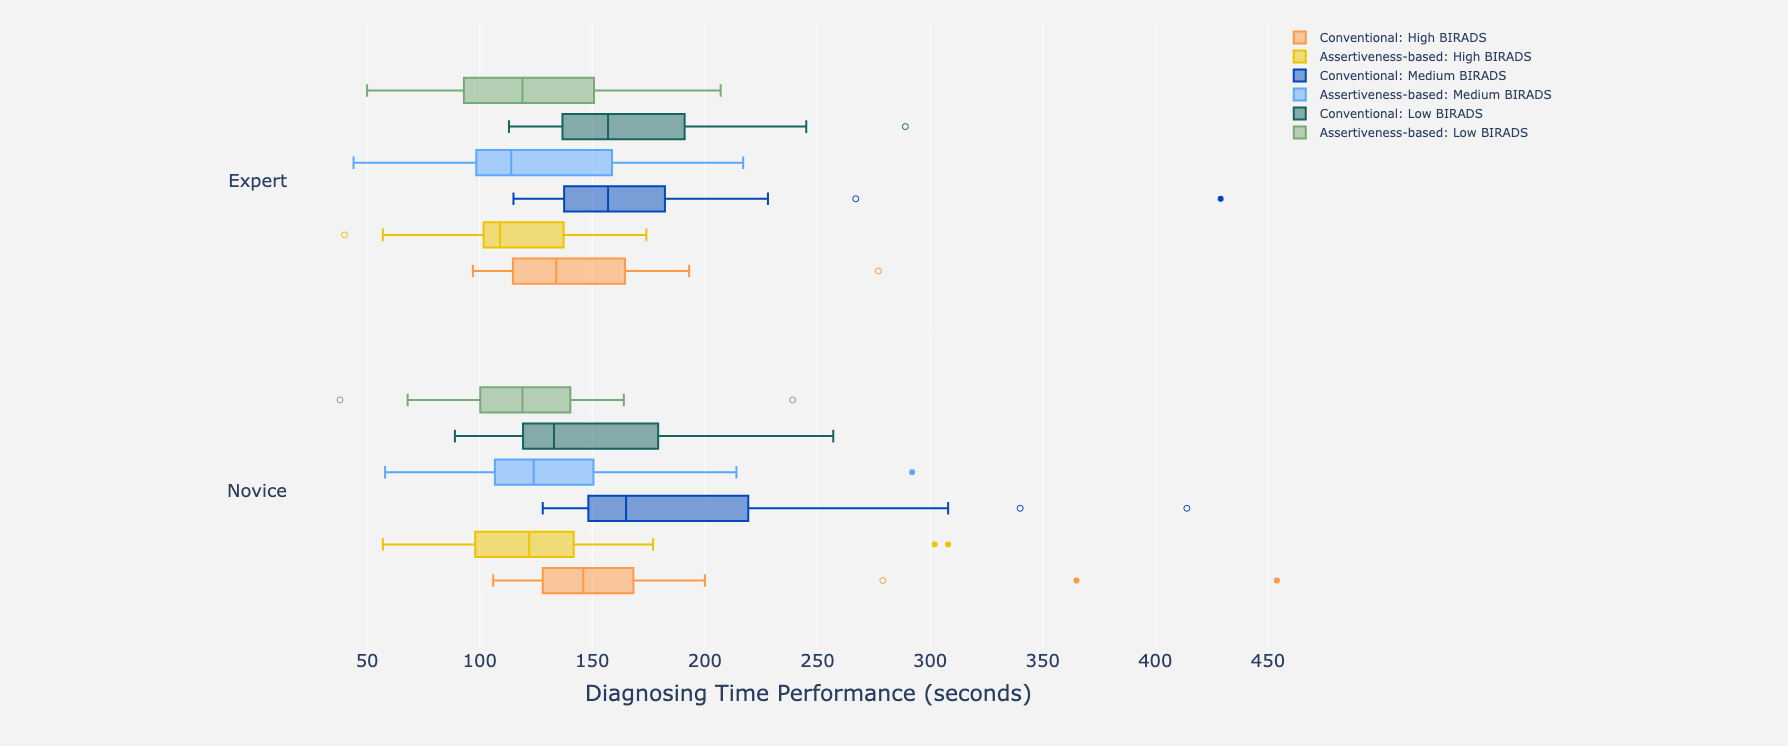
\includegraphics[width=1.000\textwidth]{fig099}
\caption[]{Diagnosing time performance in seconds of novice and expert clinicians to fully diagnose one patient. Different colors are representing different agent trials and breast severities of a patient. Clinicians' task was to read each patient and provide a final BIRADS classification by {\it accepting} or {\it rejecting} the AI recommendations.}
\label{fig:fig099}
\end{figure*}
%%%%%%%%%%%%%%%%%%%%%%%%%%%%%%%%%%%%%%%%%%%%%%%%%%%

\subsection{Analysis}
\label{sec:chap006005005}

For {\bf RQ1}, we investigated the impact of our assertiveness-based agent on clinicians' efficiency and efficacy in terms of time performance and accuracy in diagnosing patients with the support of the AI-suggested recommendations.
Similar to the literature, we used the one-way ANOVA test~\cite{SADEGHI2022105554, 10.1145/3491102.3517791} to compare both AI agents with respect to the following outcome measures per clinician:
(i) the time (in seconds) for diagnosing each patient ({\bf H1.1.}); and
(ii) accuracy rates via false-positives and false-negatives of clinician-provided classifications ({\bf H1.2.}).
For the efficacy differences between novice and expert clinicians during decision-making ({\bf H1.3.}), we used the chi-squared test of independence~\cite{10.1145/3411764.3445464} to assess the relationship between the expertise of clinicians and the assertiveness levels of the agents.
Regarding human-AI accuracy, our dataset has post-biopsy verification, meaning that we could measure the real ground-truth of the patient.

For {\bf RQ2}, we compared clinicians' perceptions of both conventional and assertiveness-based agents.
A possible observed pattern in perceived preference ({\bf H2.1.}) and trustworthiness ({\bf H2.2.}) was examined using the ANOVA test and statistical significance (p < 0.05) for testing our hypothesis.
Reported scores for cognitive workload and usability ({\bf H2.3.}) were compared between the two AI agents using statistical significance (p < 0.05) for computing the likelihood of confidence.
Last, we used the one-way ANOVA test of variance to test the levels of assertiveness for the provided clinical arguments between the two groups ({\it i.e.}, novice and expert clinicians) of medical professional experience.
Specifically, we used this test to measure the perceived preferences of clinicians in terms of reliability and capability ({\bf H2.4.}).
From ``Totally Non-Assertive'' level, {\it i.e.}, more suggestive, to ``Totally Assertive'' level, {\it i.e.}, more imposing AI recommendations, we test the overall tendency between novice and expert clinicians of the communication tone.

Finally, we used the open coding comments and feedback from focus groups, workshops, and interviews.
The purpose was to extract emerging themes from open-ended discussions during these sessions~\cite{SHIBUYA2022107131, BIEG2022107249}.
We organized the responses of clinicians using affinity diagrams to cluster workflow clinical practices and main functional ideas of the agents in greater detail~\cite{DEUTSCH2019122, 10.1145/3491101.3519863}.
Moreover, we used affinity diagramming to uncover clinicians' preferences and concerns based on the data gathered in a thematic ({\it e.g.}, card sorting) coding method.
This information was then used to inform our conclusions about exploring how to personalize and customize the AI recommendations by adapting the communication tone.

Clinicians were asked to reflect on how they used to make their decisions, what information they need to be explained by the AI models, and why they need that.
These qualitative analysis methodologies enable the identification of emerging themes in the data for revealing design considerations.
As follows (Section~\ref{sec:chap006003}), recurring themes are reported below as we detail them with provided feedback and comments from these sessions with clinicians.

\section{Results}
\label{sec:chap006006}

To test our hypotheses, we used the \texttt{scipy} library from \texttt{python} to conduct a one-way ANOVA test with the level of medical professional experience as the main factor on the dependent variables~\cite{CASALE2022107302}.
The alpha level ($\alpha$ = 0.05) was set for statistics, and the effect size was used to quantitatively measure the magnitude of the experimental comparison effect between variables~\cite{Yigit_Mendes_2018, 10.1145/3180155.3182556}.
Briefly, we focus on statistically significant results and selectively report the results to address our hypotheses by following literature recommendations~\cite{10.1145/3301275.3302289, 10.1145/3290605.3300234, 10.1145/3491102.3517791}.
Next, we investigate the time performance (Figure~\ref{fig:fig099}), accuracy (Figure~\ref{fig:fig084}) and decision (Table~\ref{tab:tab014}) rates of clinicians, while addressing their preference choices (Figure~\ref{fig:fig085}), agreement comparisons (Table~\ref{tab:tab013}), reliability and capability (Figure~\ref{fig:fig091}).

%%%%%%%%%%%%%%%%%%%%%%%%%%%%%%%%%%%%%%%%%%%%%%%%%%%
\begin{figure*}[htpb]
\centering
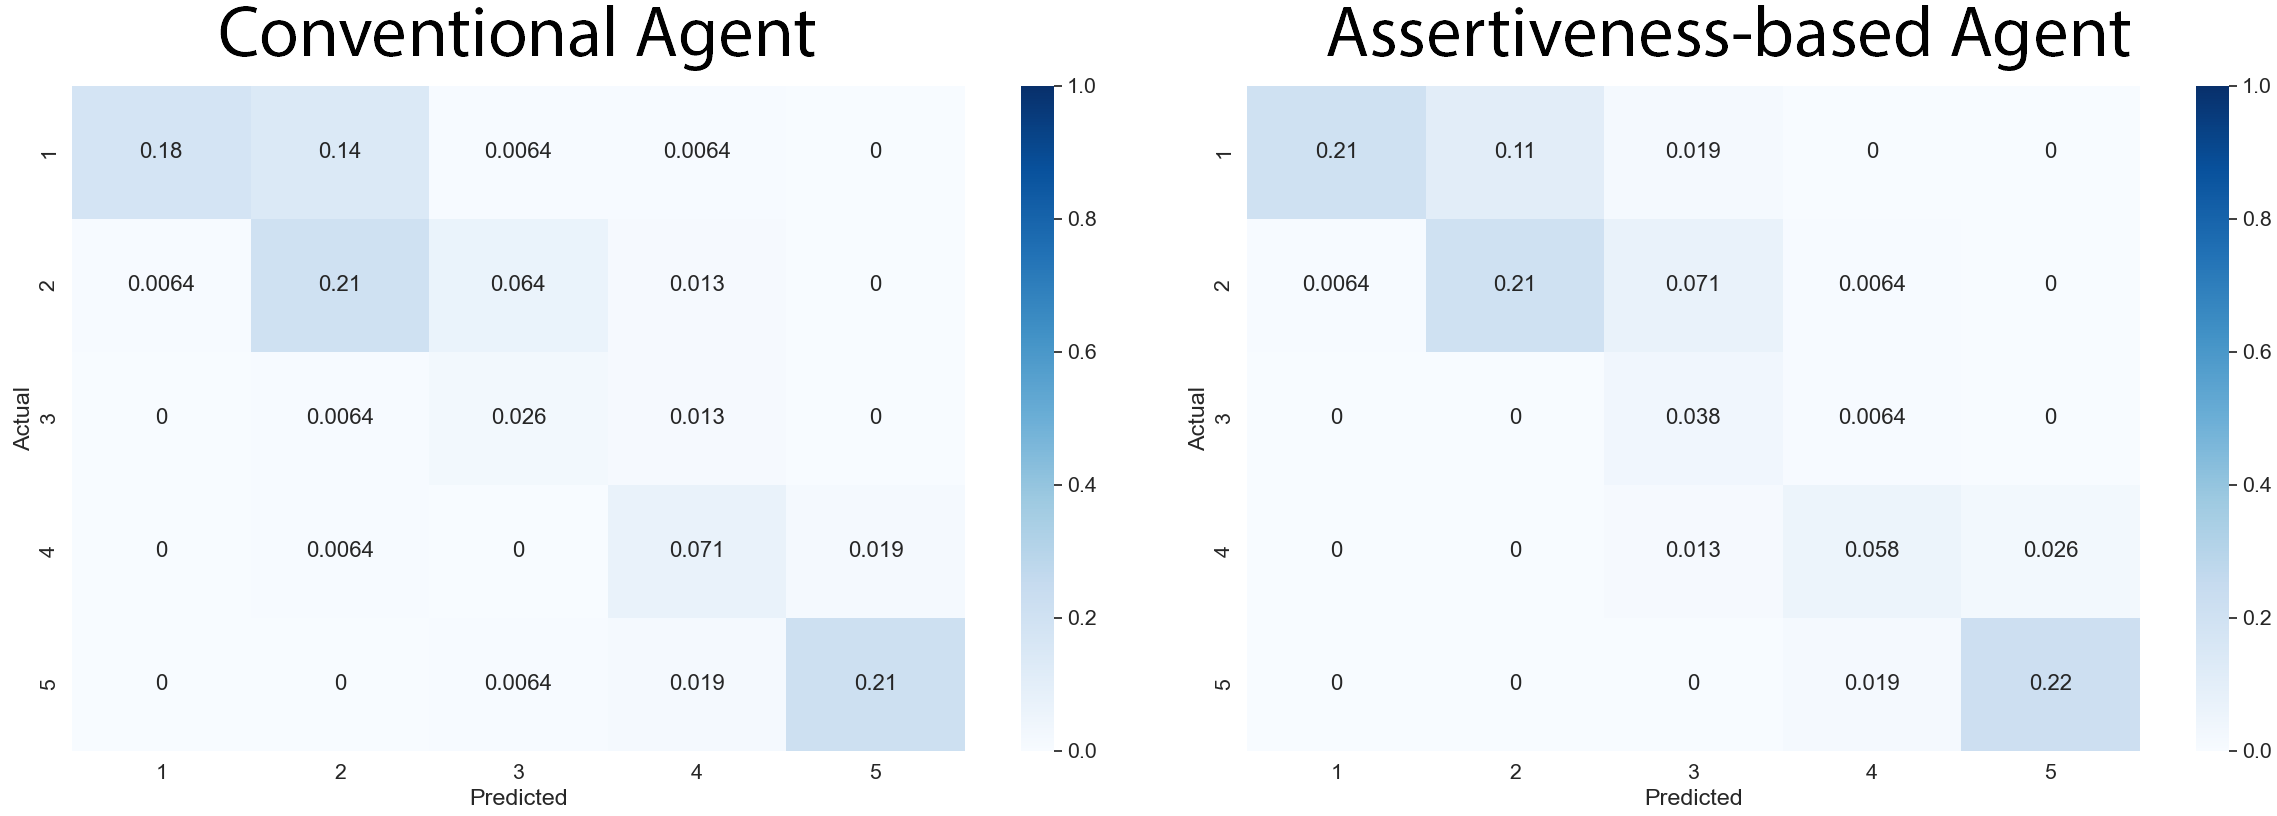
\includegraphics[width=0.855\textwidth]{fig084}
\caption[]{Accuracy rates using a confusion matrix. Comparison between the clinician's BIRADS classification (from 1 to 5) of a patient while using both conventional (left) and assertiveness-based (right) agents. Columns are representing the {\it Predicted} value (collaboration between the clinician and AI), and the rows are representing the {\it Actual} category (biopsy confirmed).}
\label{fig:fig084}
\end{figure*}
%%%%%%%%%%%%%%%%%%%%%%%%%%%%%%%%%%%%%%%%%%%%%%%%%%%

\subsection{RQ1: How does an assertiveness-based intelligent agent affect medical assessments?}
\label{sec:chap006006001}

We hypothesized that using the assertiveness-based communication between clinicians and an intelligent agent, would alter clinicians' workflow and increase the time performance of clinicians ({\bf H1.1.}) during patient diagnosis.
On average, time performance of clinicians was significantly improved with the assertiveness-based agent (M = 124.02 seconds, SD = 44.60 seconds) than with conventional agent (M = 166.12 seconds, SD = 60.42 seconds), confirming our hypothesis (Figure~\ref{fig:fig099}).
This difference was significant (F = 11.32, p = 0.005 < 0.05), indicating a large effect size (r = 0.49).

%%%%%%%%%%%%%%%%%%%%%%%%%%%%%%%%%%%%%%%%%%%%%%%%%%%
% Please add the following required packages to your document preamble:
% \usepackage{multirow}
% \usepackage{graphicx}
% \usepackage[table,xcdraw]{xcolor}
% If you use beamer only pass "xcolor=table" option, i.e. \documentclass[xcolor=table]{beamer}
\begin{table*}[bp]
\resizebox{\textwidth}{!}{%
\begin{tabular}{|c|cc|cc|cc|cc|cc|ll|}
\hline
                                     & \multicolumn{2}{c|}{\textbf{Correct Accepts}}                                        & \multicolumn{2}{c|}{\textbf{Correct Rejects}}                                      & \multicolumn{2}{c|}{\textbf{Overall Corrects}}                                       & \multicolumn{2}{c|}{\textbf{Wrong Accepts}}                                        & \multicolumn{2}{c|}{\textbf{Wrong Rejects}}                                          & \multicolumn{2}{l|}{\textbf{Overall Mistakes}}                                       \\ \cline{2-13} 
\multirow{-2}{*}{\textbf{Trials}} & \multicolumn{1}{c|}{\textbf{Novice}}                & \textbf{Expert}                & \multicolumn{1}{c|}{\textbf{Novice}}               & \textbf{Expert}               & \multicolumn{1}{c|}{\textbf{Novice}}                & \textbf{Expert}                & \multicolumn{1}{c|}{\textbf{Novice}}               & \textbf{Expert}               & \multicolumn{1}{c|}{\textbf{Novice}}                & \textbf{Expert}                & \multicolumn{1}{l|}{\textbf{Novice}}                & \textbf{Expert}                \\ \hline
\textbf{Conventional}                & \multicolumn{1}{c|}{{\color[HTML]{9A0000} 68\%}}    & {\color[HTML]{9A0000} 62\%}    & \multicolumn{1}{c|}{{\color[HTML]{9A0000} 1.7\%}}  & 1.77\%                        & \multicolumn{1}{c|}{{\color[HTML]{9A0000} 69.70\%}} & {\color[HTML]{9A0000} 63.77\%} & \multicolumn{1}{c|}{3.7\%}                         & 4.1\%                         & \multicolumn{1}{c|}{{\color[HTML]{9A0000} 26.6\%}}  & {\color[HTML]{9A0000} 32.13\%} & \multicolumn{1}{l|}{{\color[HTML]{9A0000} 30.30\%}} & {\color[HTML]{9A0000} 36.23\%} \\ \hline
\textbf{Assertive}                   & \multicolumn{1}{c|}{{\color[HTML]{009901} 79.83\%}} & 63.13\%                        & \multicolumn{1}{c|}{1.76\%}                        & {\color[HTML]{009901} 2.63\%} & \multicolumn{1}{c|}{{\color[HTML]{009901} 81.59\%}} & 65.76\%                        & \multicolumn{1}{c|}{{\color[HTML]{009901} 3.05\%}} & {\color[HTML]{9A0000} 4.75\%} & \multicolumn{1}{c|}{{\color[HTML]{009901} 15.36\%}} & {\color[HTML]{009901} 29.49\%} & \multicolumn{1}{l|}{{\color[HTML]{009901} 18.41\%}} & 34.25\%                        \\ \hline
\textbf{Non-Assertive}               & \multicolumn{1}{c|}{72.64\%}                        & {\color[HTML]{009901} 64.72\%} & \multicolumn{1}{c|}{{\color[HTML]{009901} 2.99\%}} & {\color[HTML]{9A0000} 1.69\%} & \multicolumn{1}{c|}{75.63\%}                        & {\color[HTML]{009901} 66.41\%} & \multicolumn{1}{c|}{{\color[HTML]{9A0000} 5.48\%}} & {\color[HTML]{009901} 3.91\%} & \multicolumn{1}{c|}{18.89\%}                        & 29.68\%                        & \multicolumn{1}{l|}{24.37\%}                        & {\color[HTML]{009901} 33.59\%} \\ \hline
\end{tabular}%
}
\caption[]{Frequency of clinicians, showing how often they accept or reject the AI recommendations. These rates show how often clinicians switched to a different conclusion after interacting with each agent. The ``Overall Corrects'' denote the frequency of time clinicians correctly accept (``Correct Accepts'') the recommendations of the AI agents and correctly reject (``Correct Rejects'') by changing the wrong AI recommendation to the right diagnostic. On the other hand, ``Overall Mistakes'' is denoting the frequency of times clinicians wrongly accept (``Wrong Accepts'') the AI recommendations, meaning that the AI agent was wrong, but they accept it, and wrongly reject (``Wrong Rejects''), meaning the AI agent was right, but clinicians changed to the wrong final diagnostic.}
\label{tab:tab014}
\end{table*}
%%%%%%%%%%%%%%%%%%%%%%%%%%%%%%%%%%%%%%%%%%%%%%%%%%%

We also hypothesized ({\bf H1.2.}) that using the assertiveness-based agent would not negatively affect accuracy of clinicians.
Our results show (Figure~\ref{fig:fig084}) that there was no significant difference (F = 1.85, p = 0.37 > 0.05) in accuracy.
Such results are providing support for our hypothesis ({\bf H1.2.}) that clinicians' accuracy at classifying a patient was not negatively affected by being exposed to assertiveness-based explanations.
This suggests that the assertiveness-based agent could be used in clinical settings without having a negative impact on the accuracy of patient diagnosis.
To support that claim, Table~\ref{tab:tab014} shows how often clinicians accept or reject the AI recommendations.

We further examined the potential impact of personalized explanations by customizing the agent communication differently between the two groups of professional medical experience, {\it i.e.}, novice and expert clinicians ({\bf H1.3.}).
We observed a significant association between the levels of assertiveness ({\it e.g.}, from non-assertive to assertive communication tone of the clinical arguments) and the medical professional experience while revising AI recommendations ($\chi^2$ = 3.84, p = 0.001 < 0.05).
In other words, the chance of a patient getting classified correctly by a novice was significantly higher (Accuracy\textsubscript{novice} = 91\%) with the assertive agent ({\it i.e.}, imposing AI recommendations) than with the non-assertive ({\it i.e.}, more suggestive AI recommendations).
On the contrary, the chance of correctly classifying the patient by an expert clinician was slightly higher (Accuracy\textsubscript{expert} = 78\%) with the non-assertive agent.
The odds of a patient getting classified correctly by a novice had 17.4\% chance higher with the assertive agent, while expert clinicians had 4.4\% chance higher with the non-assertive agent.
These findings suggest that the level of assertiveness of the agent's communication may need to be tailored to the experience level of the clinician.
Exploring the communication tone indicate that agents may need to be more assertive for novice clinicians, while suggestive tone may be more appropriate for expert clinicians.

Finally, Table~\ref{tab:tab014} shows how often clinicians accept or reject the AI recommendations, as well as how often they are switching to a different conclusion.
The highest overall correct rate was 81.59\% in the assertive trial for novice clinicians and 66.41\% in the non-assertive trial for expert clinicians.
Moreover, experts are switching to less wrong decisions with the non-assertive agent (Total = 33.59\%).
On the other hand, novice are switching to less wrong decisions with the assertive agent (Total = 18.41\%).
Overall, clinicians did better decisions with assertiveness-based assistance while exploring how to adapt the communication tone.
The results suggest that the assertiveness-based condition may have been more favorable to both novice and expert clinicians, with higher correct acceptance and correct reject rates compared to the conventional condition.
The results highlight the importance of scenario design in evaluating the performance of clinicians, as the trials had a significant impact on the performance of both novice and expert clinicians.

\subsection{RQ2: How is an assertiveness-based agent perceived by clinicians?}
\label{sec:chap006006002}

For RQ2, we explored clinicians' perception of both AI agents.
Results for our hypothesis ({\bf H2.1}) that clinicians would have a preference (Figure~\ref{fig:fig085}) for an assertiveness-based agent were statistically significant (F = 8.35, p = 0.001 < 0.05) between the groups of interns, juniors, middles, and seniors with a large effect size (r = 0.41).
Out of the 52 participants who expressed a preference, 66\% preferred the assertiveness-based agent and another 24\% preferred the conventional agent, while 10\% did not have a preference.

%%%%%%%%%%%%%%%%%%%%%%%%%%%%%%%%%%%%%%%%%%%%%%%%%%%
\begin{figure*}[htpb]
\centering
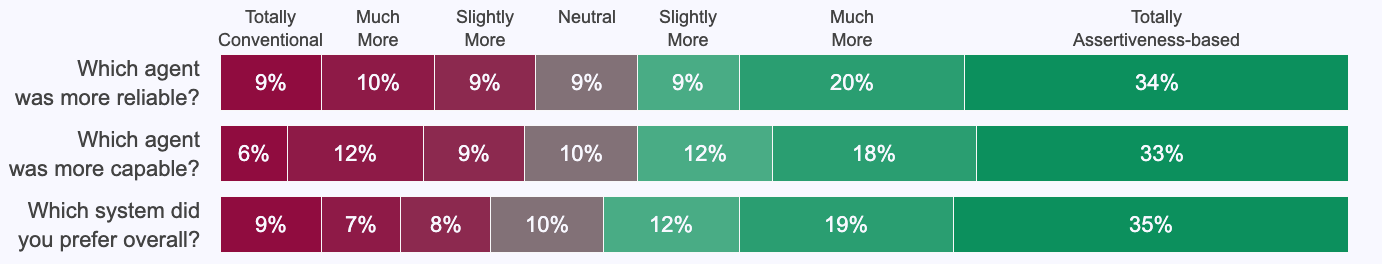
\includegraphics[width=1.000\textwidth]{fig085}
\caption[]{Preference choices of clinicians when comparing between both conventional and assertiveness-based agents within this study. Rates of clinicians are ranging from {\it Totally Conventional} to {\it Totally Assertiveness-based} on perceived {\it reliability}, {\it capability}, and {\it overall preference} of each agent.}
\label{fig:fig085}
\end{figure*}
%%%%%%%%%%%%%%%%%%%%%%%%%%%%%%%%%%%%%%%%%%%%%%%%%%%

Additional to the significant differences of preference between both conventional and assertiveness-based agents, we also analyzed perceived trust of each agent (Table~\ref{tab:tab013}).
Overall, there were only slightly differences (F = 19.47, p = 0.06 > 0.05) between conventional and assertiveness-based agents.
Besides, there were no significant differences of understanding (p = 0.14 > 0.05) between both agents.
While no significant differences in understanding could be detected between both agents, the assertiveness-based variant was considered to have greater competence (p = 0.04 < 0.05).
Moreover, we observed a trend that clinicians had higher thoughtfulness in the assertiveness-based than in the conventional agent (p = 0.001 < 0.05).
These results are providing partial support for our {\bf H2.2.} hypothesis.

We also evaluated if there were no significant differences of workload and usability between both conventional and assertiveness-based agents.
Specifically, there were no significant differences between the workload scores of the two AI agents on NASA-TLX (p = 0.38 > 0.05).
Furthermore, we observed no significant differences between the usability scores on SUS (p = 0.38 > 0.05).
Hence, providing support for our {\bf H2.3.} hypothesis for workload and usability.

%%%%%%%%%%%%%%%%%%%%%%%%%%%%%%%%%%%%%%%%%%%%%%%%%%%
\begin{table}[htpb]
\resizebox{\textwidth}{!}{%
\begin{tabular}{ccc}
\hline
Questions                                                            & Conventional & Assertiveness-based \\ \hline
Overrall, I can trust in the agent recommendations.                  & 86\%         & 90\%                \\
I understand what the system is thinking.                            & 91\%         & 94\%                \\
The system seems competent.                                          & 82\%         & 92\%                \\
The agent shows great thoughtfulness while dealing with the patient. & 71\%         & 75\%                \\ \hline
\end{tabular}%
}
\caption[]{Comparison for the percentage of agreement between conventional and assertiveness-based agents. The questions are following the three {\it dimensions of trust} represented by perceived {\it understanding}; {\it competence}; and {\it thoughtfulness}.}
\label{tab:tab013}
\end{table}
%%%%%%%%%%%%%%%%%%%%%%%%%%%%%%%%%%%%%%%%%%%%%%%%%%%

Finally, to assess how does clinicians perceive differently the levels of assertiveness (Figure~\ref{fig:fig091}), we compared the preferences in terms of reliability and capability from non-assertive (suggestive) to assertive (authoritative) communication of the clinical arguments.
Here, we can denote that there are significant differences for reliability (F = 31.36, p = 0.0001 < 0.05) and capability (F = 18.17, p = 0.0003 < 0.05) between groups of novice and expert clinicians.
In fact, novice clinicians perceived the assertive communication as more reliable (61\%), although not mainly feeling the same for capability (48\%).
On the other hand, expert clinicians perceived the non-assertive communication as more reliable (69\%) and capable (66\%).
Therefore, we can observe that the {\bf H2.4.} hypothesis is supported by showing that novice and expert clinicians will perceive differently the provided clinical arguments depending on if the agent is imposing the AI recommendations or being more suggestive.

\subsection{Qualitative Insights}
\label{sec:chap006006003}

We adopted a participatory approach for qualitatively analyzing our study results.
Given our collected data (focus group sessions, participant opinions, and transcripts), we used emergent affinity diagrams to identify common themes in how participants intend to have their clinical arguments and visualization of the AI recommendations.
Our qualitative analysis of participant responses to open-ended survey questions yielded insights on how assertiveness-based agents can affect clinicians’ workflows and their mental model.

\subsubsection{Altering Clinical Workflows}
\label{sec:chap006006003001}

To validate the proposed design, we discussed with clinicians how could they use these set of personalized agent communications to perform diagnosis on a real clinical environment.
The goal is to understand whether an assertiveness-based agent can (a) be compatible integrated into clinicians' workflow, and (b) provide added values to clinicians' diagnosis process.
Next, we summarize the main opinions of clinicians between conventional and assertiveness-based assistance, as well as between suggestive (non-assertive) and more imposing (assertive) AI recommendations.

One major criticism to the traditional approach of representing the AI recommendations with numeric BIRADS classification, accuracy of the output and heatmap values is that it is not sufficient for clinicians to make sense of the decision-making reasoning behind the output classifications.
In particular, when the output accuracy is lower than 80\% confidence.
Our qualitative findings suggest that in choosing between numeric representations of the AI output classifications and human-interpretable arguments while exploring how to adapt the communication, clinicians found the latter to be more effective during decision-making.
This highlights the necessity for AI systems to be designed with a user-centered approach~\cite{10.1145/3491102.3517789, Zimmerman2014}, taking into account the preferences and needs of the end-users (in this case, clinicians) to ensure that they are usable and effective in real-world scenarios.

\vspace{2.5mm}

\noindent
Specifically, a middle clinician ({\it i.e.}, expert clinician) reported:

\vspace{2.5mm}

\noindent
``{\it When I was interacting with the AI agents, the first thing I did was to find classification conflicts between the final BIRADS of the patient, the BIRADS of each image, output accuracy, and clinical arguments. Something that I couldn't do so well in the first [conventional] agent, but could do better for the second [assertiveness-based] one.}'' (C51)

\vspace{2.5mm}

In domains where clinicians' availability is rare, it can be exceedingly hard to obtain an immediate second reader every time a clinician needs the opinion of another human expert.
Clinicians shared a positive attitude towards the use of an assertiveness-based agent to aid their decision-making, since we are exploring how these set of agents are adapting the communication depending on the level of professional medical experience.
Something that is common when a senior (assertively) talks to an intern, while our agent is mimicking the same communication conditions.
Such mimicking behavior must be designed to help diagnosis without incurring in learning misinformation that interrupts the main clinical workflow.

%%%%%%%%%%%%%%%%%%%%%%%%%%%%%%%%%%%%%%%%%%%%%%%%%%%
\begin{figure*}[bp]
\centering
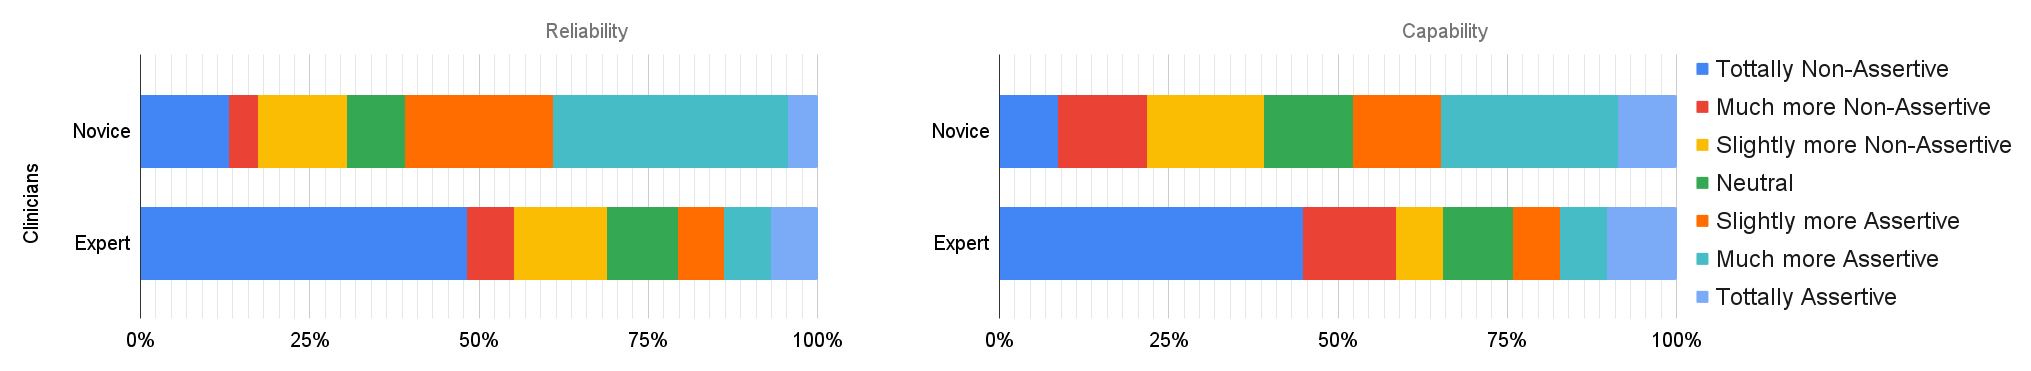
\includegraphics[width=1.000\textwidth]{fig091}
\caption[]{Ratings between novice and expert clinicians for perceived reliability and capability. Clinicians rated each agent, ranging from {\it Totally Non-Assertive} to {\it Totally Assertive} communication.}
\label{fig:fig091}
\end{figure*}
%%%%%%%%%%%%%%%%%%%%%%%%%%%%%%%%%%%%%%%%%%%%%%%%%%%

\noindent
Here, a senior clinician ({\it i.e.}, expert clinician) is sustaining the above argument by reporting that:

\vspace{2.5mm}

\noindent
``{\it Adapting the communication between more suggestive [non-assertive] or assertive tone of the clinical arguments can help the diagnosis workflow. I may prefer a suggestive agent, but an assertive agent will be more helpful for my interns concerning an educational purpose.}'' (C15)

\vspace{2.5mm}

Categorically, clinicians were mostly stating that they could understand how such personalized communication could be beneficial to customize the interaction between humans and AI.
In particular, clinicians valued the opportunity to choose the communication tone to explore the clinical arguments in a more detailed fashion.
Our qualitative findings suggest that most clinicians (48/52) found the assertiveness-based agent to be more helpful and reliable.
These findings also support our claim that customization could have a positive impact on the decision-making process and improve the overall effectiveness of AI-assisted systems.

\vspace{2.5mm}

\noindent
As another example, a junior clinician ({\it i.e.}, novice clinician) reported that:

\vspace{2.5mm}

\noindent
``{\it When the agent is talking to me in a more assertive way, I can feel more safe of my decision... and feeling more assurance of the right answer.}'' (C17)

\vspace{2.5mm}

This analysis further highlights the effectiveness of the assertiveness-based agent in personalizing and customizing the communication of the agent, taking into account differences of medical professional experience.
That is, 37 out of 52 clinicians in our study explicitly mentioned that their workflow differed between the two agents.
Particularly, clinicians showed different confidence and trusting opinions depending on the levels of assertiveness.

\vspace{2.5mm}

\noindent
For instance, an intern clinician ({\it i.e.}, novice clinician) reported that:

\vspace{2.5mm}

\noindent
``{\it It seems like, when I was interacting with the more suggestive [non-assertive] assistant, it has the same doubts on the communication tone as I am. The more assertive assistant gave me higher confidence in the decision.}'' (C10)

\vspace{2.5mm}

\noindent
On the other hand, a senior clinician ({\it i.e.}, expert clinician) reported the following:

\vspace{2.5mm}

\noindent
``{\it In my opinion, I don't like the communication tone and the way assertive agents are reporting the clinical arguments. Imposing the AI recommendations feels like I need to follow the orders they give to me. I prefer a more suggestive agent, asking me if the clinical arguments are well classified or not.}'' (C49)

\vspace{2.5mm}

To conclude, these levels of personalizing and customizing the agent communication ({\it e.g.}, from less assertive to more assertive) are important to take into account when designing systems for critical domains.
Especially, for decision-making under these clinical workflows.
We found that assertiveness-based not only enhanced decision-making, but also helped clinicians to develop a mental model of the AI agents, or probe for the likelihood of the diagnosis.
Next, we describe in what manner our work is leveraging these insights.

\subsubsection{Agent Mental Models}
\label{sec:chap006006003002}

Both novice and expert clinicians have preconceived mental models about the levels of assertiveness in different ways.
As an example, expert clinicians used the output results to disambiguate AI errors from their own errors, depending on the communication tone.
It is, therefore, possible that this reasoning behavior is projected onto the AI agent to anticipate where the agent would likely make mistakes: ``{\it It could be also important to adapt the communication tone of the clinical arguments depending on the AI confidence.}''
From here, we could understand that expert clinicians expect that the assertiveness of a clinical argument can also be adapted depending on the accuracy of the AI output results for that particular variable.
On the contrary, novice clinicians were more focused on the learning process and patient comparisons for educational purpose: ``{\it For me, the most important thing was to look at the provided arguments and understand if they are right from what I learn or from similar cases. A junior like me must have an idea how the machine is thinking to mentally follow the same reasoning process from my side.}''
Hence, it is important to provide a more `{\it storytelling-like}' view of the patient for novice clinicians, even though in a more assertive fashion.

Apart from preconceptions, we further observed that clinicians developed comparative mental models between conventional and assertiveness-based agents: ``{\it The first AI [assertiveness-based] was outstanding… but in the second AI [conventional] I was frustrated with the lack of communication in comparison to the first one.}''
Moreover, the interaction experience of clinicians with the different AI agents can also shape their reasoning while looking for AI recommendation mistakes: ``{\it In the second assistant [assertiveness-based], I look for classification conflicts between the final BIRADS and the clinical arguments, while I couldn't do the same for the first assistant [conventional], taking me more time to see if there are some mistakes.}''

Our intelligent agents can leverage these insights by not only provide a personalized and customized communication with different perspectives between novice and expert clinicians, but also correction behavior while adjusting internal representations of specific levels of assertiveness. Yet, without hurting time performance of the diagnostic (Section~\ref{sec:chap006001}), nor increasing the workload (Section~\ref{sec:chap006002}).
In sum, these observations support growing evidence that taking into account the communication of the AI outputs ({\it e.g.}, structure, order, and tone of the arguments) can alter the clinicians' perceptions of the mental models of assisting agents.

\section{Discussion}
\label{sec:chap006007}

In this work, we studied how personalized and customized communication of an intelligent agent can aid clinicians in their decision-making during medical imaging diagnosis.
We conducted a within-subject to investigate how clinicians perceive assertiveness-based agents differently.
Our results are showing that assertiveness-based agents can alter clinicians' workflows by increasing the efficiency of clinicians while maintaining overall efficacy.

Overall, the classification accuracy was not affected by providing assertiveness-based communication.
We observed a significant effect of differences between novice and expert clinicians, depending on the explanations tone.
This promising insight motivates future directions in the development and validation of compliant agents, capable of providing relevant and customized explanations.

Participants were keener on following AI recommendations that adapt their communication tone than the one that did not.
Although this effect may occur because of adding more explanations, it reflected in differences of behavioral decisions between novice and expert clinicians.
We gain even more insight on the effect of tone from the feedback provided by the clinicians across our qualitative analysis.
Our qualitative results are showing that participants appreciate the idea of adapting tone to probe the likelihood of the diagnosis.
This finding might be in line with the previous research in psychology and decision support science~\cite{LOMBROZO2010303, 10.1093/mind/fzu023, Seidel2021}, bringing new directions for the theoretical application of assertiveness-based communication in deep learning systems and clinical domains.

We studied how personalizing and customizing the AI recommendations according to the professional experience of each clinician can reduce medical errors and increase satisfaction.
Specifically, we found significant differences in terms of accuracy, perceived reliability and capability between novice and expert clinicians, depending on the tone of the personalized explanations.
This finding is relevant in the design of AI agents for the healthcare sector, while providing a contribution to the HCI field.

Clinicians' overall preferences and perceived trust were also increased for the assertiveness-based agent in comparison with the conventional.
Results suggest a higher perceived understanding of the assertiveness-based agent compared to the conventional variant.
On the same hand, the assertiveness-based agent showed to be perceived by clinicians as more competent and thoughtful.
However, our results are indicating the existence of other latent variables.
For instance, the demographic characteristics of clinicians with different levels of clinical experience could shape the implementation of intelligent agents to take into account the differences in clinicians' perception of AI systems generally.

In terms of results significance for the HCI community, our research focuses on the use of intelligent agents in medical imaging, which is an important and growing area within HCI.
By developing personalized and customized explanations, we aim to improve the effectiveness of decision-making by human clinicians, which is a key concern in HCI.
Our specific contribution to the CHI community is the design of a novel interactive approach for personalized and customized explanations on intelligent agents, underpinned by computational principles.
Our approach combines machine learning with image processing techniques to generate explanations that are tailored to the individual clinician's expertise.
To our knowledge, this is the first time that this approach has been proposed and evaluated in the context of medical imaging.

Concerning the broader implications of our work, we believe that it has relevance for both decision support research and AI communication research.
Our approach to personalized and customized explanations has the potential to improve the accuracy and effectiveness of decision-making by humans in critical domains, which is an essential goal in decision-support research.
At the same time, our work also contributes to the growing body of research on how to improve the communication between AI systems and human users, which is a key concern in AI communication research.
Next, we are discussing the design implications and generalizability of our findings, by concluding the limitations of our study and directions for future work.

\subsection{Design Implications}
\label{sec:chap006007001}

Our findings have different stages of design implications for the development of novel AI-assisted systems in this clinical domain.
Presented findings are ranging from the combination of different knowledge classifiers of the clinical arguments, training these models with enriched information, to the design of user interfaces for embedded intelligent agents.
In addition, it is important to conduct further research to explore the potential benefits and limitations of different knowledge representation methods and to evaluate the effectiveness of different design features in enhancing the performance of AI systems.
Ultimately, our findings aim to inform the development of more human-centered medical AI systems that effectively support clinical decision-making and enhance patient outcomes.
As follows, we will provide our recommendations to inform future work on human-centered medical AI systems.

\subsubsection{Different Knowledge Combination}
\label{sec:chap006007001001}

In a real clinical workflow, extra patient information is necessary for a proper breast cancer diagnosis.
Providing the lesion details and relevance of the classification is an important functionality for better decision-making.
From our interviews, we learn that such information is crucial for diagnostic speed and accuracy, as it informs the clinician on what to look for and where to find the lesions.
To better match the AI with the mental model of clinicians and provide better guidance, as well as explanations, we should incorporate granular patient information from the model classifiers~\cite{doi:10.1148/ryai.210299}.
For instance, the AI might use different classifiers to provide information on the lesion contours, whereas other classifiers are focused on the lesion margins.
This assumption takes us to another recommendation, how should we train the models with such mixed information, for proper integration into real clinical workflows.

\subsubsection{Training Mixed Models}
\label{sec:chap006007001002}

Our study suggests that clinical workflows and trust can be positively affected by endowing personalization of the agent communication.
In fact, with the ability to, not only incorporate granular patient information from the mixed model classifiers, but also adapt the tone depending on the medical experience of the clinician.
Implementation of such intelligent agents would require that DL models are equipped with the additional prediction of mixed clinical arguments ({\it e.g.}, lesion contours, margin, or cancer type of the patient) beyond diagnosis alone.
This additional granular information about the patient could include its importance to the diagnostic, while also customizing the communication tone depending on the various demographic characteristics of clinicians.
Such an idea could be integrated either into one fused training, or by developing multi separated models, one for each clinical variable.
% Such an idea could be integrated either into one fused training~\cite{cortez2021fullyautomated}, or by developing multi separated models, one for each clinical variable~\cite{ALANTARI201844}.

\subsubsection{Adapting Communication}
\label{sec:chap006007001003}

In this work, we evaluate one specific way of personalizing and customizing the communication between agents and clinicians with different levels of medical experience.
We did that by exploring how to adapt the communication tone depending on if the agent was communicating with a novice or an expert clinician.
While our results suggest that this communication technique may be effective, we recommend that future work may explore different demographic characteristics of clinicians.
For example, from different medical institutions ({\it e.g.}, public hospitals, private clinics, cancer centers, etc), or different medical fields ({\it e.g.}, family physicians, breast surgeons, etc.), where some behavioral decision-making of clinicians should differ.
Besides, our qualitative results (Section~\ref{sec:chap006006002}) are showing that clinicians are also willing for adapting the communication tone of the clinical arguments depending on the AI confidence.
For instance, if confidence is greater than 80\%, then the system should display an Assertive recommendation (Figure~\ref{fig:fig098}, middle).
Otherwise, it should display a Non-Assertive recommendation (Figure~\ref{fig:fig098}, bottom).
As a research direction, we should explore how different performance actions of the intelligent agents will impact behavioral decision-making of clinicians.

\subsubsection{Generalizability}
\label{sec:chap006007001004}

Through this exploration, our study sheds light on the use of assertiveness-based agents in the specific domain of breast cancer based on medical imaging diagnosis.
It is important to note that the results of our study should not be generalized to other medical domains without caution.
Hence, we warn in generalizing the results of this study to other domains.
However, we argue that similar communication techniques of personalized and customized explanations can be useful for various types of medical diagnosis because the challenges motivating our study are common across several other medical specialties.

Despite our focus on the breast cancer domain, this demographic characteristics of clinicians ({\it i.e.}, differences in behavioral decision-making between novice and expert) is transversal to other applications~\cite{STAHNKE2021103243, LANDRO2020102897, doi:10.1080/21642850.2020.1741372}.
Such claim is making our approach useful beyond the specific domain of breast cancer diagnosis.
For instance, lung cancer diagnosis requires that specialized radiologists visually inspect chest imaging data similar in nature to that used in our study~\cite{10.1145/3313831.3376807}.
In both of these fields, it may be valuable to personalize and customize the agent communication, depending on their background and expertise, leading to more accurate diagnoses and improved patient outcomes.

The potential of personalizing and customizing the agent communication depending on the levels of medical experience can also be addressed for other clinical domains.
As another example, in skin cancer some works are trying to mimic the medical procedures, where clinicians rely on their past experience across similar cases to reach the final diagnosis~\cite{10.1007/978-3-030-87199-4_52, Tschandl2020, Esteva2017}.
Depending on the past experience of that clinician, the agent should adapt the provided information and communication to them, or other customizable techniques.
Others are stating that AI-based systems must be improved with personalized medicine supporting diagnosis and treatment guidance~\cite{Sollini2020, Aerts2016, IBRAHIM2019438}.
These studies suggest that the recommendations we make for medical imaging diagnosis in this work have been considered independently and may be of merit beyond the development of assertiveness-based agents.

% Hence, it is important to provide a more `{\it storytelling-like}' view of the patient for novice clinicians, even though in a more assertive fashion.

% \clearpage

\subsection{Limitations and Future Work}
\label{sec:chap006007002}

In this work, we conducted a within-subject experiment to investigate the use of assertiveness-based agents by clinicians in the particular medical domain of breast cancer diagnosis.
We investigate this question through the design and study of Assertiveness-based BreastScreening-AI.
More specifically, this tool was used to explore how an intelligent agent should adapt its communication tone depending on the professional experience ({\it i.e.}, novice vs expert) of the clinician.

Due to the short availability of clinicians and the remote nature of our study, it was challenging to control the tasks of each step in the experiment precisely.
For example, participants varied how long they complete the task for the first patient, in comparison to the second and third patients.
This lack in experimental control may have impacted the degree to which exposure to the first patient, while interacting for the first time with the assertiveness-based agent, affected how clinicians interacted with the latter.

Another limitation is related with the implications of liability when using AI in medical settings~\cite{10.1145/3555157}, where the legal framework for addressing these issues is still evolving.
The use of AI in medical settings raises complex questions that are not yet fully understood or addressed by existing laws and regulations~\cite{10.1145/3411764.3445432}.
This can make it difficult to determine who might be liable in the event of an error or harm caused by an AI system.
AI systems often operate in complex and dynamic environments, making it challenging to identify the specific factors that led to a particular outcome.
Overall, the limitations concerning the implications of liability when using AI in medical settings highlight the need for further research and legal developments in this area.
It is important for policymakers and other stakeholders to continue to explore these issues and work to address them in a way that ensures the safe and effective use of AI in medical settings.

In our study, the assertiveness-based agent was using specific AI outputs, curated and selected by us alongside choosing the most typical clinical setups in a real-world environment.
While prior work has demonstrated the potential of predicting the likelihood of a clinician to trust on an AI recommendation from raw medical data~\cite{pmlr-v97-raghu19a}, future work should focus on training DL models based on personalized and customized explanations to provide human-interpretable arguments for clinicians.

As another future direction, we will study the effects of the two different main features of the assertiveness-based agent ({\it i.e.}, explanations and tone), in more conditions separately (Section~\ref{sec:app001007}).
However, inferring useful information for adapting the DL model, presents new technical challenges for the AI community.
For the HCI community, the challenge is making such inferences transparent, considering some behavioral characteristics of clinicians.

\section{Conclusion}
\label{sec:chap006008}

In this work, we provide a novel perspective on how to personalize and customize the explanations of intelligent agents to human clinicians.
Our results from an experimental study with 52 clinicians comparing a conventional agent to an assertiveness-based agent suggest that the ability of a system to not only exploring how to adapt the communication tone ({\it i.e.}, more suggestive or more assertive), but also provide granular explanations of patient cases has merits for end users.
From our results, the time performance was satisfactory, where clinicians took less 25\% of the time to diagnose a patient with the assertiveness-based agent in comparison to the conventional agent.
As we observed, the caparison between the conventional agent and the assertiveness-based agent was more effective also with the latter in achieving the proper diagnostic of the patient.
Additionally, our results demonstrate that if explanations are adapted taking into account the medical experience of clinicians, accuracy chance of correctly diagnosing a patient is 91\% higher for novice and 78\% higher for expert clinicians.
Last, clinicians are showing an increase of trust, preferring the assertiveness-based agent by being more reliable and capable, as this agent was revealing to be further understandable, competent and thoughtful.
Our work has implications for the design of AI systems not only in the medical domains, but also in fields that are facing similar challenges, demanding a personalization of the human-AI interaction.